\documentclass[11pt,a4paper]{article}
\usepackage[T1]{fontenc}
\usepackage[utf8]{inputenc}
\usepackage{lmodern}
\usepackage{microtype}
\usepackage[margin=27mm,headheight=15pt]{geometry}
\usepackage{amsmath,amssymb,amsthm,mathtools}
\usepackage{booktabs,array,longtable}
\usepackage{graphicx}
\usepackage{xcolor}
\usepackage{enumitem}
\usepackage{fancyhdr}
\usepackage{xurl}
\usepackage[colorlinks=true,linkcolor=blue!45!black,citecolor=blue!45!black,urlcolor=blue!45!black]{hyperref}
\hypersetup{pdftitle={Sharp Codimension Thresholds and Uniform Amplification on the Boolean Cube},pdfauthor={Research manuscript prepared with ChatGPT for ProveIt},pdfsubject={Boolean Fourier analysis, conditional variance, stability, exact certificates}}
\newcommand{\E}{\mathbb E}
\newcommand{\Pbb}{\mathbb P}
\newcommand{\R}{\mathbb R}
\newcommand{\Z}{\mathbb Z}
\newcommand{\N}{\mathbb N}
\newcommand{\1}{\mathbf 1}
\newcommand{\Var}{\operatorname{Var}}
\newcommand{\Law}{\mathcal L}
\newcommand{\TV}{d_{\mathrm{TV}}}
\newcommand{\degc}{\operatorname{cdeg}}
\newcommand{\sgn}{\operatorname{sign}}
\newcommand{\Bin}{\operatorname{Bin}}
\newcommand{\Inf}{\operatorname{Inf}}
\newcommand{\supp}{\operatorname{supp}}
\newcommand{\Q}{\mathbb Q}
\newcommand{\dist}{\operatorname{dist}}
\newtheorem{theorem}{Theorem}[section]
\newtheorem{lemma}[theorem]{Lemma}
\newtheorem{proposition}[theorem]{Proposition}
\newtheorem{corollary}[theorem]{Corollary}
\newtheorem{claim}[theorem]{Claim}
\theoremstyle{definition}
\newtheorem{definition}[theorem]{Definition}
\newtheorem{example}[theorem]{Example}
\newtheorem{question}[theorem]{Question}
\theoremstyle{remark}
\newtheorem{remark}[theorem]{Remark}
\numberwithin{equation}{section}
\setlist{topsep=5pt,itemsep=3pt,parsep=0pt}
\setlength{\parskip}{3pt}
\setlength{\emergencystretch}{2em}
\pagestyle{fancy}
\fancyhf{}
\fancyhead[L]{\small Sharp codimension thresholds on the Boolean cube}
\fancyfoot[C]{\thepage}
\renewcommand{\headrulewidth}{0.3pt}
\title{\textbf{Sharp Codimension Thresholds and Uniform\\
Amplification on the Boolean Cube}\\[8pt]
\large A twenty-bit witness, distributional rigidity,\\
and exact research certificates}
\author{Research manuscript prepared for the ProveIt repository\\
\small Generated with ChatGPT (GPT-6 Astra Pro)}
\date{7 October 2026}
\begin{document}
\maketitle
\begin{abstract}
For a finite observation \(F\) of \(N\) independent uniform signs, let
\(D(F)\) be the largest Fourier degree of one of its cell indicators and
\(v(F)=\Var(\E[H_N\mid F])\), where \(H_N\) is the coordinate sum.
Building on the observation framework in the OpenAI manuscript
\emph{Unbounded Violations of the Square-Root Degree Bound}, we determine
the first Fourier codimension at which \(v(F)\le D(F)\) can fail.
If every cell has degree at most \(N-k\), with \(k=1,2,3\), then every
conditional coordinate-sum variance is at least \(k\). Equality holds
exactly for translated \(k\)-sign-sum laws. We prove quantitative
total-variation stability, including sharp local moduli in the associated
alternating-moment class.

At codimension four, an explicit partition of the twenty-dimensional cube
has 622 cells, exact cell degree 16, and retained variance
\(16+9/34816\). Its exceptional cell has 8704 points and conditional
variance \(4-9/289\). All values are certified by exact rational
arithmetic. Tensor products yield additive gaps growing linearly with
the number of copies. An exhaustive certificate also proves twenty-bit
minimality within a precisely specified binomial-block reporting family.

Finally, we quantify the source manuscript's normal-approximation
amplifier: one fixed averaging count works at every stage, and explicit
degree and dimension bounds follow. A rational Gaussian parameter choice
gives a positive, albeit extremely small, numerical exponent. The
existence of a power separation itself is already a consequence of the
source result and balanced Boolean composition; the quantitative
construction is distinguished from that prior consequence.
The article includes complete proofs, reproducible certificates, a
repository integration plan, and a further research agenda.
\end{abstract}
\vspace{5pt}
\noindent\textbf{Keywords.}
Boolean Fourier analysis; conditional expectation; polynomial degree;
binomial laws; stability; exact computation.

\noindent\textbf{Verification status.}
The proofs are mathematical arguments accompanied by exact finite
certificates. They have not been formalized or checked by Lean.
Priority claims are limited to comparison with the inspected sources.
\clearpage
\begingroup
\small
\setlength{\parskip}{0pt}
\tableofcontents
\endgroup
\newpage
\section{Research context and the results}
\label{sec:context}

The useful common ground between the two repositories is finite Fourier
analysis with explicit verification. The OpenAI manuscript
\emph{Unbounded Violations of the Square-Root Degree Bound}
\cite{OpenAI2026} develops low-degree observations whose conditional
coordinate sums retain unexpectedly large variance. ProveIt's
\emph{Noisy parity cubes} report \cite{ProveItNoise} studies spectral
samples, parity noise, and query costs, while its Thue--Morse Lean files
\cite{ProveItWalsh} establish finite character identities. This article
uses the former observation mechanism, develops a new structural
threshold and rigidity theory, and follows the latter repository's
practice of separating written proofs from finite computational checks.

\subsection{What was reviewed}

The OpenAI repository catalog and overview were examined to choose a
focused problem. The proof-level review for this article covers all seven
section files of result family 192: the observation calculus, reporting
construction, alternative reports, mean-cost extension, weighted
Gaussian mixture, and small-width calculation. The fixed source revision
is
\[
\texttt{adc7f1241b42e322a6451854ab7e4b4c146bf78a}.
\]
The ProveIt review covers the actual source of \emph{Noisy parity cubes},
its verification script, and the two Lean files
\texttt{ThueMorseBooleanCube.lean} and \texttt{ThueMorseWalsh.lean}, at
revision
\[
\texttt{dfc1a5a6817462e0465e445e1466c41ee42ea839}.
\]
The repository README was also inspected at the later snapshot
\texttt{1aa2f12ec85b}.
These are scoped mathematical reviews, not audits of every result in
either repository. Exact paths and source identities are recorded in the
accompanying provenance file.

Theorem 3.1 of \emph{Noisy parity cubes} represents a Boolean rule's
two-input disagreement under independent XOR noise as a mixture of the
corresponding parity disagreement probabilities, with squared Walsh
coefficients as weights. Its Lemma 3.2 compares total influence with
expected exact query cost. Those conclusions concern noise response and
queries; they do not imply a variance bound for arbitrary low-degree
cells. The inspected Lean files prove product identities and vanishing
nontrivial Walsh-character sums in a binary representation. They do not formalize the
conditional-expectation results proved here.

\subsection{The distinction between three Fourier quantities}

For \(f:\{-1,1\}^N\to\{-1,1\}\), write
\[
 L(f)=\sum_{i=1}^N\widehat f(\{i\}),\qquad
 L_{\mathrm{abs}}(f)=\sum_{i=1}^N|\widehat f(\{i\})|.
\]
These differ from the squared first-level Fourier weight and from total
influence. Coordinate sign changes preserve degree and turn the signed
sum into the absolute sum. Thus their universal extremal inequalities
are equivalent, although the values for a particular function need not
be equal.

The Gopalan--Servedio problem asks whether \(L(f)\le\sqrt{\deg f}\);
O'Donnell's problem list records it and the stronger majority benchmark
\(L(f)\le B_{\deg f}\), where \(B_d=\E|H_d|\)
\cite{ODonnell2012}. The same square-root question appears as
Conjecture 3.17 in \cite{FHKL2016}. The source manuscript
\cite{OpenAI2026} proves violations by every constant factor. The
present article does not claim that prior conclusion as a new theorem.

For coordinate-subcube partitions, the retained variance equals the
expected number of fixed coordinates. This is the conditional-sum
calculation behind the decision-tree inequality of O'Donnell and
Servedio \cite[Theorem 3]{ODonnellServedio2007}. Blais, Tan, and Wan
\cite[Lemma 3.1]{BlaisTanWan2015} use the same type of conditional sum
for parity decision trees. General low-degree indicators allow
cancellation unavailable to coordinate subcubes. The codimension
question asks how far that cancellation can first go.

\subsection{The structural threshold}

Let \(D(F)\) denote maximum cell degree, as defined precisely in
Section~\ref{sec:observations}. The principal result is the following.

\begin{theorem}[First possible codimension for a variance gain]
\label{thm:headline}
Let \(X_1,\ldots,X_N\) be independent uniform signs and
\(H_N=\sum_iX_i\).
\begin{enumerate}
\item If \(C\ne\varnothing\) and
\(\deg\1_C\le N-k\), where \(k\in\{1,2,3\}\), then
\[
 \Var(H_N\mid C)\ge k.
\]
Equality holds if and only if \(\Law(H_N\mid C)\) is an integer translate
of the law of a sum of \(k\) independent uniform signs.
\item Consequently, if \(D(F)\le N-k\), then \(v(F)\le N-k\).
Equality holds if and only if every attained cell has the equality
distribution in the first assertion.
\item There is an explicit twenty-bit observation \(F_*\) with
\[
 D(F_*)=16,\qquad
 v(F_*)=16+\frac9{34816}.
\]
Its exceptional cell \(A\) has exact degree 16 and
\[
 \Var(H_{20}\mid A)=4-\frac9{289}.
\]
\end{enumerate}
Thus four is the smallest Fourier codimension \(N-D(F)\) at which
retained variance can exceed cell degree.
\end{theorem}

The first two assertions are proved using interlacing even and odd
integer lattices. The last is a completely specified finite example,
not a limiting construction. Its numerical excess is small, but it
locates an exact boundary that the qualitative amplifier does not
identify.

The equality statement is distributional. It does not classify a cell
as a coordinate subcube. Indeed, the proof only requires certain
alternating moments of the Hamming-weight distribution to vanish.
The stability theorem makes this distinction quantitative. If
\(\Delta=(N-k)-v(F)\), then for suitable integer shifts \(c(F)\) and an
independent \(k\)-sign sum \(S_k\),
\begin{equation}\label{eq:headline-stability}
 \TV\bigl(\Law(F,H_N),\Law(F,c(F)+S_k)\bigr)
 \le C_k\Delta,\qquad
 (C_1,C_2,C_3)=\left(\frac14,\frac14,\frac38\right).
\end{equation}
We also prove sharper local bounds and construct extremizers in the
abstract moment class.

\subsection{Other contributions and their scope}

The finite reporter is reduced to an exact rational optimization
formula, and its full score law is computed as a four-atom perturbation
of \(H_{16}\). Tensorization proves that no universal additive constant
can repair \(v(F)\le D(F)\). Exhaustive rational enumeration proves
twenty-bit minimality within the family of equal binomial blocks,
sum-level leaf tests, and a central-sum selector. This is not a
classification of every observation on fewer than twenty bits.

For the source Gaussian amplifier, we prove explicit restricted-moment
estimates, a uniform fourth-moment invariant, and a single copy count
valid at every iteration. The resulting construction has polynomial
dimension growth in its prescribed degree budget. A fully rational
choice supplies the numerical exponent
\(\varepsilon_0=2^{-8\,000\,000\,000}\).
Its size makes the construction an effective existence theorem rather
than a practical way to tabulate a counterexample.

There is a necessary priority distinction here. Once an arbitrary-factor
square-root violation is known, balanced block composition already
implies a positive power separation. Fact 2.7 of
\cite{BlaisTanWan2015} gives the relevant multiplication rule.
Section~\ref{subsec:composition} proves the short deduction, including
the balancing step. The additional content of our analytic construction
is the fixed quantitative schedule and explicit constants, not the bare
existence of a positive exponent.

All main mathematical claims are proved below. Their priority relative
to the entire literature remains a matter for further scholarly review;
the comparison here is with the repository sources and primary papers
actually inspected.

\section{Finite observations and exact degree bookkeeping}
\label{sec:observations}

The probability measure on \(\{-1,1\}^N\) is uniform. For
\(S\subseteq[N]\), put \(\chi_S(x)=\prod_{i\in S}x_i\). Every real
function \(g\) has the expansion
\[
 g=\sum_{S\subseteq[N]}\widehat g(S)\chi_S,\qquad
 \widehat g(S)=\E[g\chi_S],
\]
and its Fourier degree is the largest \(|S|\) with
\(\widehat g(S)\ne0\). Nonzero constant functions have degree zero;
zero indicators can be discarded throughout.

\begin{definition}
A finite observation is a function \(F:\{-1,1\}^N\to\mathcal A\) with
finite range. Its cells are the nonempty sets \(C_a=\{F=a\}\). Define
\[
 D(F)=\degc(F)=\max_{\Pbb(F=a)>0}\deg\1_{C_a},\quad
 T_F=\E[H_N\mid F],\quad
 v(F)=\E T_F^2.
\]
The quantity \(N-D(F)\) is the \emph{Fourier codimension} of the
observation. It is a deficit of polynomial degree, not the geometric
codimension of its cells.
\end{definition}

Since \(\E H_N=0\), the score \(T_F\) is centered. Orthogonal projection,
or a direct cellwise expansion of the square, gives
\begin{equation}\label{eq:total-variance}
 N=v(F)+\E\Var(H_N\mid F).
\end{equation}
In particular \(0\le v(F)\le N\).

\begin{lemma}[Observation calculus]\label{lem:observation-calculus}
Every function of \(F\) has degree at most \(D(F)\). If \(F_i\) are
observations on disjoint blocks with degrees \(D_i\), then every
function of their tuple has degree at most \(\sum_iD_i\).
For the tuple itself, its exact cell degree is \(\sum_iD_i\), and its
retained variance is \(\sum_iv(F_i)\).
\end{lemma}

\begin{proof}
Expand a function of \(F\) as
\(\sum_a g(a)\1_{C_a}\). On disjoint blocks, a cell of the tuple is a
product of cell indicators, so its degree is at most the sum of the
degrees. Conversely, choose in each factor a cell of maximal degree
and a nonzero coefficient of that degree. Their product is a nonzero
coefficient on the disjoint union of the corresponding supports.
Hence the sum is attained. Independence gives
\[
 \E[H_{\mathrm{tot}}\mid(F_i)_i]=\sum_iT_{F_i}.
\]
The scores are independent and centered, proving variance additivity.
\end{proof}

If \(Q\) is any coarsening of the tuple, the tower property gives
\begin{equation}\label{eq:tower-scores}
 \E[H_{\mathrm{tot}}\mid Q]=
 \E\left[\sum_i T_{F_i}\,\middle|\,Q\right].
\end{equation}
Score collisions cause no degree difficulty: merging labels merely
adds their indicators.

\begin{lemma}[Boolean readout and the surviving linear bound]
\label{lem:readout}
Let \(v(F)>0\), put \(\kappa(F)=\E T_F^4/v(F)^2\), and define
\(f=\sgn(T_F)\), with \(\sgn(0)=1\). Then
\[
 \deg f\le D(F),\qquad
 L(f)=\E|T_F|\ge\sqrt{\frac{v(F)}{\kappa(F)}}.
\]
For every Boolean function \(g\),
\begin{equation}\label{eq:linear-bound}
 L_{\mathrm{abs}}(g)\le I(g)\le\deg g,
\end{equation}
where \(I(g)\) is total influence.
\end{lemma}

\begin{proof}
The degree assertion is Lemma~\ref{lem:observation-calculus}. Since
\(f\) is a function of \(F\),
\[
 L(f)=\E[fH_N]=\E[fT_F]=\E|T_F|.
\]
Hölder's inequality applied to
\(|T|^2=|T|^{2/3}|T|^{4/3}\) gives
\[
 \E T^2\le(\E|T|)^{2/3}(\E T^4)^{1/3},
\]
which rearranges to the desired bound.

For the last assertion define the discrete derivative
\[
 \partial_i g(x_{\ne i})
 =\frac{g(x_{\ne i},1)-g(x_{\ne i},-1)}2.
\]
It takes values in \(\{-1,0,1\}\), has mean
\(\widehat g(\{i\})\), and has second moment \(\Inf_i(g)\).
Thus \(|\widehat g(\{i\})|\le\Inf_i(g)\).
Orthogonality gives
\[
 I(g)=\sum_S|S|\widehat g(S)^2
 \le(\deg g)\sum_S\widehat g(S)^2=\deg g.
\]
This familiar inequality is also recorded in
\cite{NisanSzegedy1994,ODonnell2012}.
\end{proof}

A retained-variance excess \(v(F)>D(F)\) is therefore an intermediate
structural fact. It alone does not ensure that the sign readout
violates \(L(f)\le\sqrt{\deg f}\), because the first absolute moment
depends on the shape of the score distribution. Our twenty-bit example
makes this distinction concrete.

\section{Sharp codimension barriers and distributional stability}
\label{codim:section}

The Fourier-degree condition imposes useful restrictions on each cell
separately.  For the first three codimensions, these restrictions determine
the least possible conditional variance of the coordinate sum.  They also
give a quantitative description of every cell whose variance is close to
that minimum.  The description concerns a probability distribution:
different cells can have the same distribution of the coordinate sum
without having the same geometry.

\subsection{Alternating moments and two interlaced lattices}

\begin{lemma}[Alternating-moment cancellation]
\label{codim:alternating}
Let \(1\le k\le N\), let \(C\subseteq\{-1,1\}^N\) have positive
uniform probability, and suppose
\(\deg\1_C\le N-k\).  For
\[
Y=\frac{N-H_N}{2},
\]
one has
\begin{equation}
\label{codim:alternating-equation}
\E[(-1)^Y Y^j\mid C]=0
\qquad(0\le j<k).
\end{equation}
In particular, conditional on \(C\), the even and odd values of \(Y\)
each have probability \(1/2\).  Their normalized conditional
distributions have identical moments through order \(k-1\).
\end{lemma}

\begin{proof}
The variable \(Y\) counts the negative coordinates, so
\[
(-1)^Y=\chi_{[N]}(X).
\]
The function \(Y^j\), after multilinear reduction on the cube, has
Fourier degree at most \(j\).  Multiplication by \(\chi_{[N]}\)
takes \(\chi_S\) to \(\chi_{[N]\setminus S}\).  Thus
\(\chi_{[N]}Y^j\) has Fourier support only at degrees at least
\(N-j>N-k\).  Orthogonality of the Walsh characters gives
\[
\E[\1_C\chi_{[N]}Y^j]=0.
\]
Division by \(\Pbb(C)>0\) proves
\eqref{codim:alternating-equation}.

The equation for \(j=0\) gives parity balance.  For any subsequent
\(j\), the same equation says that the unnormalized \(j\)-th moments
on the two parity classes agree.  Since the classes each have mass
\(1/2\), their normalized moments agree as well.
\end{proof}

The following elementary fact supplies the needed variance estimates.
Its equality condition will be used repeatedly.

\begin{lemma}[Variance on a lattice of spacing two]
\label{codim:lattice}
Suppose \(Z\) takes values in \(a+2\Z\), has finite second moment,
and has mean \(\mu\in[a,a+2]\).  Then
\begin{equation}
\label{codim:lattice-bound}
\Var(Z)\ge(\mu-a)(a+2-\mu).
\end{equation}
Equality holds if and only if \(Z\) is supported on
\(\{a,a+2\}\).  In that case its probabilities are necessarily
\((a+2-\mu)/2\) and \((\mu-a)/2\).
\end{lemma}

\begin{proof}
For every \(z\in a+2\Z\), the product
\((z-a)(z-a-2)\) is nonnegative and vanishes exactly at \(a,a+2\).
Taking expectations and expanding gives
\[
0\le \E[(Z-a)(Z-a-2)]
=\Var(Z)-(\mu-a)(a+2-\mu).
\]
The equality statement follows from pointwise nonnegativity.
The mean determines the two probabilities.
\end{proof}

\begin{proposition}[The first three alternating-moment bounds]
\label{codim:moment-variance}
Let \(k\in\{1,2,3\}\), and let \(Y\) be integer valued with finite
second moment and
\begin{equation}
\label{codim:abstract-moments}
\E[(-1)^Y Y^j]=0
\qquad(0\le j<k).
\end{equation}
Then
\[
\Var(Y)\ge k/4.
\]
Equality holds if and only if
\[
\Law(Y)=\Law(m+B_k)
\]
for some integer \(m\), where \(B_k\) has distribution
\(\operatorname{Bin}(k,1/2)\).
\end{proposition}

\begin{proof}
Translation by an integer preserves
\eqref{codim:abstract-moments}: the parity factor changes by a constant
sign, and a translated \(j\)-th power is a polynomial of degree at most
\(j\).  We can therefore translate the mean to an interval convenient
for the proof.

For \(k=1\), translate so that \(\mu=\E Y\in[0,1]\).  Each parity
has mass \(1/2\).  The nearest even lattice point to \(\mu\) is \(0\),
and the nearest odd lattice point is \(1\), with a possible tie at an
endpoint.  Hence
\[
\Var(Y)
\ge \frac12\mu^2+\frac12(1-\mu)^2
=\frac14+(\mu-1/2)^2.
\]
Equality at \(1/4\) forces \(\mu=1/2\), and then forces the even
and odd conditional laws to be point masses at \(0\) and \(1\).
This is \(B_1\).

For \(k\ge2\), the conditional means on the two parity classes
agree.  Write their common mean as \(\mu\), and translate it to
\(u\in[0,1]\).  The even and odd conditional variances, denoted by
\(V_e,V_o\), satisfy
\begin{equation}
\label{codim:AB}
V_e\ge A(u):=u(2-u),
\qquad
V_o\ge B(u):=1-u^2,
\end{equation}
by Lemma~\ref{codim:lattice}, using the pairs \(\{0,2\}\) and
\(\{-1,1\}\), respectively.

For \(k=2\), the equality of conditional means gives
\[
\Var(Y)=\frac{V_e+V_o}{2}
\ge\frac12+u-u^2
\ge\frac12.
\]
Equality requires \(u=0\) or \(u=1\), together with equality in
both lattice bounds.  At \(u=0\), the even law is the point mass at
\(0\), and the odd law has equal masses at \(-1,1\).
The full law has weights \((1,2,1)/4\) on \(-1,0,1\).
The case \(u=1\) is its integer translate.  These are precisely
the translates of \(B_2\).

For \(k=3\), the conditional second moments agree in addition to
the means, so
\[
V_e=V_o=\Var(Y).
\]
Consequently
\[
\Var(Y)\ge\max\{A(u),B(u)\}
=\frac34+|u-1/2|-|u-1/2|^2
\ge\frac34.
\]
Since \(|u-1/2|\le1/2\), equality at \(3/4\) forces \(u=1/2\).
Equality in both instances of Lemma~\ref{codim:lattice} then gives
the full probabilities
\[
\frac18,\quad\frac38,\quad\frac38,\quad\frac18
\]
on \(-1,0,1,2\), which is \(B_3-1\).

Conversely, every translate of \(B_k\) has variance \(k/4\)
and satisfies the required cancellations.  For the latter assertion,
\[
\E[(-1)^{B_k}z^{B_k}]=2^{-k}(1-z)^k;
\]
applying \((z\,d/dz)^j\) and evaluating at \(z=1\) gives zero for
\(j<k\).  Integer translation preserves these cancellations.
\end{proof}

\begin{theorem}[Cellwise variance barrier]
\label{codim:barrier}
Let \(k\in\{1,2,3\}\), let \(N\ge k\), and suppose
\(D(F)\le N-k\).  Every attained cell \(C=\{F=a\}\) satisfies
\begin{equation}
\label{codim:cell-barrier}
\Var(H_N\mid F=a)\ge k.
\end{equation}
Therefore
\begin{equation}
\label{codim:retained-barrier}
v(F)\le N-k.
\end{equation}
Equality in \eqref{codim:cell-barrier} holds exactly when the
conditional law of \(H_N\) is an integer translate of the sum of
\(k\) independent uniform signs.  Equality in
\eqref{codim:retained-barrier} holds exactly when this condition holds
in every attained cell, with a possibly different translate in each
cell.  Revealing any \(N-k\) coordinates attains equality.
\end{theorem}

\begin{proof}
Lemma~\ref{codim:alternating} and
Proposition~\ref{codim:moment-variance} apply to
\(Y=(N-H_N)/2\) in each cell.  Since
\(\Var(H_N\mid C)=4\Var(Y\mid C)\), they prove the cellwise
bound and its equality characterization.  More explicitly, if
\(Y\mid C\) has law \(m+B_k\), then
\[
H_N\mid C\ \stackrel{\rm law}{=}\
N-2m-k+S_k,
\]
where \(S_k=k-2B_k\) is a sum of \(k\) uniform signs.
The translate consequently has the parity required by the original
cube.

The total variance identity gives
\[
N=\Var(H_N)
=v(F)+\E[\Var(H_N\mid F)].
\]
A finite positive-weight average of quantities each at least \(k\)
equals \(k\) if and only if every quantity equals \(k\).  This proves
the retained-variance statement and its equality condition.
Finally, after \(N-k\) coordinates are revealed, the remaining
\(k\) signs are independent and uniform.  The cell indicators have
degree \(N-k\), and the conditional variance is exactly \(k\).
\end{proof}

\begin{corollary}[Bounds that retain the conditional mean]
\label{codim:mean-sensitive}
Let \(C\) be a cell as in Lemma~\ref{codim:alternating}, and let
\(u\in[0,1]\) be the fractional part of
\(\E[(N-H_N)/2\mid C]\).  For \(k=2\),
\begin{equation}
\label{codim:mean-two}
\Var(H_N\mid C)\ge2+4u(1-u).
\end{equation}
For \(k=3\),
\begin{equation}
\label{codim:mean-three}
\Var(H_N\mid C)
\ge3+4|u-1/2|-4|u-1/2|^2.
\end{equation}
\end{corollary}

\begin{proof}
These are the two estimates before minimization over \(u\) in the
proof of Proposition~\ref{codim:moment-variance}, multiplied by four.
\end{proof}

\begin{figure}[tb]
\centering
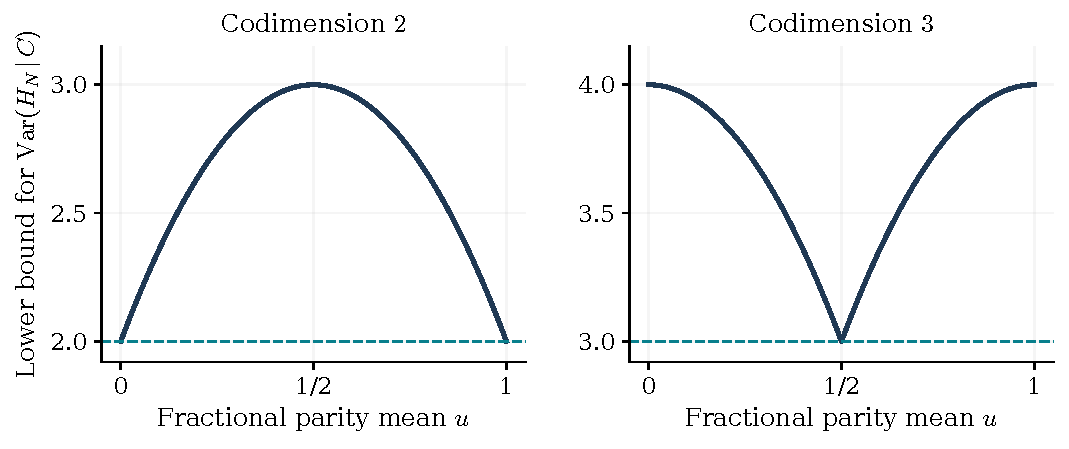
\includegraphics[width=.94\linewidth]{figures/parity_bounds.pdf}
\caption{The mean-sensitive conditional-variance bounds. The fractional
part \(u\) of the common parity-conditioned Hamming-weight mean
controls the extra variance forced by the two interlacing lattices.
Dashed lines mark the universal minima.}
\label{fig:parity-bounds}
\end{figure}

\begin{remark}
All the preceding assertions hold for a signed coordinate sum
\(\sum_i\epsilon_iX_i\), with fixed \(\epsilon_i\in\{-1,1\}\).
The change of variables \(X_i\mapsto\epsilon_iX_i\) preserves the
uniform law and every Fourier degree.  The equality statements
classify the conditional laws of these sums; they do not characterize
which coordinates a cell fixes.
\end{remark}

\subsection{A stable projection onto neighboring lattice points}

We use the convention
\[
\TV(P,Q)=\frac12\sum_{z\in\Z}|P\{z\}-Q\{z\}|.
\]
Here and below, \(\delta_z\) denotes a unit point mass at \(z\).
The next estimate controls the entire distribution by the slack in
Lemma~\ref{codim:lattice}.

\begin{lemma}[Stable lattice projection]
\label{stab:lattice-projection}
Under the hypotheses of Lemma~\ref{codim:lattice}, set
\[
Q_\mu=\frac{a+2-\mu}{2}\delta_a+
      \frac{\mu-a}{2}\delta_{a+2}.
\]
Then
\begin{equation}
\label{stab:projection-bound}
\TV(\Law(Z),Q_\mu)
\le\frac14\left\{
\Var(Z)-(\mu-a)(a+2-\mu)
\right\}.
\end{equation}
Moreover,
\begin{equation}
\label{stab:outside-bound}
\Pbb\{Z\notin\{a,a+2\}\}
\le\frac18\left\{
\Var(Z)-(\mu-a)(a+2-\mu)
\right\}.
\end{equation}
\end{lemma}

\begin{proof}
Put \(J=(Z-a)/2\) and \(t=\E J\in[0,1]\).  The slack, divided
by four, is
\[
S=\E[J(J-1)]\ge0.
\]
Let
\[
q=\Pbb\{J\notin\{0,1\}\},
\qquad
b=\E[J\1_{\{J\notin\{0,1\}\}}].
\]
The differences between the actual masses at \(0,1\) and the target
masses \(1-t,t\) are \(b-q,-b\), respectively.  Therefore
\[
\TV\bigl(\Law(J),(1-t)\delta_0+t\delta_1\bigr)
=\frac{q+|b-q|+|b|}{2}
=\max\{q,b,q-b\}.
\]
For every integer \(j\notin\{0,1\}\),
\[
1\le j(j-1),\qquad
j\le j(j-1),\qquad
1-j\le j(j-1).
\]
Their expectations give \(q,b,q-b\le S\), proving
\eqref{stab:projection-bound}.  Finally,
\(j(j-1)\ge2\) outside \(\{0,1\}\), so \(q\le S/2\).
This proves \eqref{stab:outside-bound}.
\end{proof}

\subsection{Quantitative stability near the three variance minima}

\begin{definition}
\label{stab:distance-definition}
For an integer-valued random variable \(Y\), define its distance from
the binomial translates by
\[
d_k(Y)=\inf_{m\in\Z}
\TV\bigl(\Law(Y),\Law(m+B_k)\bigr),
\qquad B_k\sim\operatorname{Bin}(k,1/2).
\]
For \(0\le\delta\le1/4\), write
\[
r(\delta)=\frac{1-\sqrt{1-4\delta}}2.
\]
Thus \(0\le r(\delta)\le1/2\) and
\(r(\delta)-r(\delta)^2=\delta\).
\end{definition}

\begin{theorem}[Linear stability, with explicit local moduli]
\label{stab:main}
Let \(Y\) satisfy the assumptions of
Proposition~\ref{codim:moment-variance}, and put
\(\delta=\Var(Y)-k/4\ge0\).  For \(k=1,2\),
\begin{equation}
\label{stab:global-twelve}
d_k(Y)\le\delta.
\end{equation}
For \(k=3\),
\begin{equation}
\label{stab:global-three}
d_3(Y)\le\frac32\delta.
\end{equation}
When \(0\le\delta\le1/4\), the stronger bounds are
\begin{align}
d_k(Y)&\le\frac12r(\delta)
=\frac{1-\sqrt{1-4\delta}}4,
&& k=1,2,
\label{stab:local-twelve}\\
d_3(Y)&\le\frac34r(\delta)
=\frac38\bigl(1-\sqrt{1-4\delta}\bigr).
\label{stab:local-three}
\end{align}
In particular,
\begin{equation}
\label{stab:small-three}
d_3(Y)\le\delta
\qquad(0\le\delta\le3/16).
\end{equation}
Every bound is obtained by an explicitly chosen integer translate.
\end{theorem}

\begin{proof}
Integer translation and reflection preserve the alternating-moment
conditions.  They also preserve \(d_k\), since \(k-B_k\) and \(B_k\)
have the same law.  We use these operations to normalize the mean.

\paragraph{The case \(k=1\).}
Translate so that \(u=\E Y\in[0,1]\), and put
\(a=|u-1/2|\le1/2\).  Then
\[
S:=\E[Y(Y-1)]
=\Var(Y)+u^2-u
=\delta+a^2.
\]
Let \(b(y)\) be \(0\) or \(1\) according to the parity of the
integer \(y\).  Parity balance gives \(\E b(Y)=1/2\).
For every integer \(y\),
\[
|y-b(y)|\le y(y-1).
\]
For \(y=0,1\) both sides vanish; for all other integers the
inequality follows immediately by considering \(y\le-1\) and
\(y\ge2\).  Consequently
\[
a=|\E[Y-b(Y)]|\le S,
\qquad
\delta\ge a-a^2.
\]
Every single atom of \(Y\) has mass at most \(1/2\).  Thus its
distance from \((\delta_0+\delta_1)/2\) is exactly
\(q=\Pbb\{Y\notin\{0,1\}\}\).
Since \(y(y-1)\ge2\) outside those two integers,
\begin{equation}
\label{stab:one-intermediate}
d_1(Y)\le q\le\frac{\delta+a^2}{2}.
\end{equation}
Because \(a\le1/2\), we have
\(\delta\ge a-a^2\ge a^2\), which proves
\eqref{stab:global-twelve} for \(k=1\).
If \(\delta\le1/4\), the monotonicity of \(x-x^2\) on
\([0,1/2]\) gives \(a\le r(\delta)\).  Substituting this in
\eqref{stab:one-intermediate} and using
\(\delta+r(\delta)^2=r(\delta)\) proves
\eqref{stab:local-twelve}.

\paragraph{Common notation for \(k=2,3\).}
The parity-conditioned means agree.  After translation, suppose their
common value is \(u\in[0,1]\), and define
\[
Q_e^u=(1-u/2)\delta_0+(u/2)\delta_2,
\qquad
Q_o^u=((1-u)/2)\delta_{-1}+((1+u)/2)\delta_1.
\]
Their variances are \(A(u),B(u)\) from \eqref{codim:AB}.
Their equally weighted mixture is
\begin{equation}
\label{stab:nu}
\nu_u=
\frac{1-u}{4}\delta_{-1}
+\frac{2-u}{4}\delta_0
+\frac{1+u}{4}\delta_1
+\frac{u}{4}\delta_2.
\end{equation}
The even and odd supports are disjoint, so
Lemma~\ref{stab:lattice-projection} gives
\begin{equation}
\label{stab:mixture-projection}
\TV(\Law(Y),\nu_u)
\le\frac{V_e-A(u)+V_o-B(u)}8.
\end{equation}

\paragraph{The case \(k=2\).}
Choose the nearest integer to the common mean, translate to that
integer, and reflect if necessary.  We then have \(u\in[0,1/2]\).
Since
\(\Var(Y)=(V_e+V_o)/2=1/2+\delta\), the two nonnegative
lattice slacks yield
\[
\delta\ge u-u^2,
\qquad
\TV(\Law(Y),\nu_u)
\le\frac{\delta-u+u^2}{4}.
\]
The law \(\nu_0\) is that of \(B_2-1\).
Direct comparison in \eqref{stab:nu} gives
\(\TV(\nu_u,\nu_0)=u/2\).  Hence
\begin{equation}
\label{stab:two-intermediate}
d_2(Y)\le\frac{\delta+u+u^2}{4}.
\end{equation}
For \(0\le u\le1/2\),
\[
u+u^2\le3(u-u^2)\le3\delta,
\]
which proves the global bound.  If \(\delta\le1/4\),
then \(u\le r(\delta)\), and
\eqref{stab:two-intermediate} becomes
\[
d_2(Y)\le\frac{\delta+r(\delta)+r(\delta)^2}{4}
=\frac12r(\delta).
\]

\paragraph{The case \(k=3\).}
Translate the common parity mean to \(u\in[0,1]\), and put
\(a=|u-1/2|\).  Here
\(V_e=V_o=3/4+\delta\), and \eqref{codim:AB} gives
\[
\delta\ge a-a^2.
\]
Since \(A(u)+B(u)=3/2-2a^2\),
\eqref{stab:mixture-projection} reads
\[
\TV(\Law(Y),\nu_u)\le\frac{\delta+a^2}{4}.
\]
The law \(\nu_{1/2}\) is that of \(B_3-1\), and
\(\TV(\nu_u,\nu_{1/2})=a/2\).  We obtain
\begin{equation}
\label{stab:three-intermediate}
d_3(Y)\le\frac{\delta+a^2+2a}{4}.
\end{equation}
For \(a\in[0,1/2]\),
\[
a^2+2a\le5(a-a^2)\le5\delta,
\]
proving \eqref{stab:global-three}.
When \(\delta\le1/4\), we have \(a\le r(\delta)\), and
\eqref{stab:three-intermediate} gives
\[
d_3(Y)\le
\frac{\delta+r(\delta)^2+2r(\delta)}4
=\frac34r(\delta).
\]
Finally, if \(\delta\le3/16\), then \(a\le r(\delta)\le1/4\),
and the stronger inequality
\[
a^2+2a\le3(a-a^2)\le3\delta
\]
in \eqref{stab:three-intermediate} proves
\eqref{stab:small-three}.
\end{proof}

\subsection{Sharpness in the alternating-moment class}

We record exact families attaining the local estimates.  Their role is
to identify the best possible modulus under the stated moment
conditions.  An additional realization argument would be needed to
assert the same optimality among uniform laws on Fourier-degree
constrained cube cells.

\begin{proposition}[Sharp local moduli]
\label{stab:sharpness}
The bounds \eqref{stab:local-twelve} are attained for every
\(0\le\delta\le1/4\).  The bound \eqref{stab:local-three} is
attained for every \(0\le\delta\le3/16\).  Thus the leading constants
\(1/2,1/2,3/4\) in front of \(\delta\) are optimal in the
alternating-moment class for \(k=1,2,3\), respectively.
\end{proposition}

\begin{proof}
First note a separation fact.  Any two distinct integer translates
of \(B_k\) are at TV distance at least its largest atom.  Indeed,
let \(j_*\) be a largest atom, and compare \(B_k\) with \(B_k+h\),
where \(h\ge1\).  On the event \((-\infty,j_*]\), the difference
of their probabilities is
\[
\Pbb\{j_*-h<B_k\le j_*\}\ge\Pbb\{B_k=j_*\}.
\]
Negative shifts are reduced to positive ones by translation and
symmetry of TV.  The largest atom equals \(1/2\) for \(k=1,2\)
and \(3/8\) for \(k=3\).  Consequently, whenever a law is at
distance at most half this separation from one translate, no other
translate can be closer: this follows from the triangle inequality.

For \(k=1\), let \(0\le t\le1/2\), and take
\[
\Pbb\{Y=0\}=(1-t)/2,\qquad
\Pbb\{Y=1\}=1/2,\qquad
\Pbb\{Y=2\}=t/2.
\]
Parity balance holds.  The mean and second moment are
\(1/2+t\) and \(1/2+2t\), so
\[
\Var(Y)=1/4+t-t^2.
\]
Its distance from \(B_1\) is \(t/2\le1/4\), making \(B_1\)
a nearest translate by the separation fact.

For \(k=2\), take \(Y\) with law \(\nu_t\) from
\eqref{stab:nu}, again with \(0\le t\le1/2\).
Each parity has mass \(1/2\), and both conditional means are \(t\).
The second moment is \(1/2+t\), whence
\[
\Var(Y)=1/2+t-t^2.
\]
Its distance from \(B_2-1=\nu_0\) is \(t/2\le1/4\).
This translate is therefore nearest.

For \(k=3\), let \(0\le t\le1/4\), and use the five-point law
\begin{equation}
\label{stab:sharp-three-family}
\begin{array}{c|ccccc}
y&-3&-1&0&1&2\\ \hline
\Pbb\{Y=y\}
&t/8&1/8-t/2&3/8-t/4&3/8+3t/8&1/8+t/4 .
\end{array}
\end{equation}
All its probabilities are nonnegative and sum to one.  The even
and odd classes each have mass \(1/2\).  Their normalized first
moments both equal \(1/2+t\), and their normalized second moments
both equal \(1+2t\).  Thus all three required alternating moments
vanish, and
\[
\Var(Y)=1+2t-(1/2+t)^2=3/4+t-t^2.
\]
Relative to \(B_3-1\), the positive mass differences occur at
\(-3,1,2\), and sum to
\[
t/8+3t/8+t/4=3t/4.
\]
This is at most \(3/16\), so the displayed binomial translate is
nearest.

In all three families, \(\delta=t-t^2\), hence
\(t=r(\delta)\).  The first two parameter intervals cover
\(\delta\in[0,1/4]\); the third covers \(\delta\in[0,3/16]\).
These are exactly the stated attainment ranges.
Finally \(r(\delta)=\delta+O(\delta^2)\) as
\(\delta\downarrow0\), which proves the assertion about leading
constants.
\end{proof}

\subsection{From cellwise stability to the joint observation law}

\begin{corollary}[Stability in the coordinate-sum normalization]
\label{stab:cell}
Under the cell hypotheses of Theorem~\ref{codim:barrier}, suppose
\[
\Var(H_N\mid C)\le k+\varepsilon
\]
for some \(\varepsilon\ge0\).
There is an integer \(c\equiv N-k\pmod2\) such that
\[
\TV\bigl(\Law(H_N\mid C),\Law(c+S_k)\bigr)
\le
\begin{cases}
\varepsilon/4,&k=1,2,\\
3\varepsilon/8,&k=3.
\end{cases}
\]
If \(0\le\varepsilon\le1\), the respective stronger bounds are
\[
\frac{1-\sqrt{1-\varepsilon}}4
\quad(k=1,2),
\qquad
\frac38\bigl(1-\sqrt{1-\varepsilon}\bigr)
\quad(k=3).
\]
For \(k=3\) and \(\varepsilon\le3/4\), the bound
\(\varepsilon/4\) is valid as well.
\end{corollary}

\begin{proof}
Apply Theorem~\ref{stab:main} to the conditional law of
\(Y=(N-H_N)/2\), for which
\[
0\le\delta=\Var(Y\mid C)-k/4\le\varepsilon/4.
\]
All the displayed bounding functions are increasing on their stated
domains.  TV is unchanged under the bijection \(y\mapsto N-2y\)
from \(\Z\) onto the parity lattice \(N+2\Z\).
The binomial translate \(m+B_k\) is sent to
\(c+S_k\), where \(c=N-2m-k\).  This also proves the parity
assertion.
\end{proof}

\begin{corollary}[Joint-law stability near saturation]
\label{stab:joint}
Let \(k\in\{1,2,3\}\), suppose \(D(F)\le N-k\), and put
\[
\Delta=(N-k)-v(F)\ge0.
\]
There is an integer-valued function \(c\) of the attained labels of
\(F\), with \(c(a)\equiv N-k\pmod2\), such that
\begin{equation}
\label{stab:joint-bound}
\TV\bigl(\Law(F,H_N),\Law(F,c(F)+S_k)\bigr)
\le C_k\Delta,
\qquad
C_1=C_2=\frac14,\quad C_3=\frac38,
\end{equation}
where \(S_k\) is independent of \(F\).
For \(k=3\), one may replace \(C_3\) by \(1/4\) if every attained
cell satisfies
\(\Var(H_N\mid F=a)\le3+3/4\).
\end{corollary}

\begin{proof}
For each attained label \(a\), let
\[
\varepsilon_a=\Var(H_N\mid F=a)-k\ge0
\]
and choose \(c(a)\) by Corollary~\ref{stab:cell}.  The observation
has finitely many attained labels, so this defines the desired function
without a selection issue.  Construct the comparison law using the
same \(F\)-marginal and an independent \(S_k\).
For two joint laws with the same first marginal, direct summation of
the absolute differences gives
\begin{align*}
&\TV\bigl(\Law(F,H_N),\Law(F,c(F)+S_k)\bigr)\\
&\qquad=
\sum_a\Pbb\{F=a\}
\TV\bigl(\Law(H_N\mid F=a),\Law(c(a)+S_k)\bigr)\\
&\qquad\le C_k\sum_a\Pbb\{F=a\}\varepsilon_a.
\end{align*}
The last sum is
\[
\E[\Var(H_N\mid F)]-k
=N-v(F)-k=\Delta.
\]
This proves \eqref{stab:joint-bound}.  The additional cellwise
hypothesis permits the improved constant in
Corollary~\ref{stab:cell} for every summand.
\end{proof}

\begin{remark}
The model in \eqref{stab:joint-bound} is a mixture of translated
\(k\)-sign sums with a quantitatively controlled error.  Applying the
projection \((a,h)\mapsto h\) gives the same bound for the
unconditional coordinate-sum marginals.  Neither conclusion asserts
that the observation is close to a coordinate-revealing map or that
its cells are close to subcubes.  Controlling such geometric features
would require additional information beyond the law of the sum.
\end{remark}

\subsection{The fourth-order moment relaxation}

The alternating-moment condition alone changes character at the next
order.  The following proposition concerns an abstract moment class;
it supplies no construction of a cube cell.

\begin{proposition}[The order-four relaxation]
\label{codim:four-relaxation}
Among integer-valued laws with finite third absolute moment satisfying
\[
\E[(-1)^Y Y^j]=0\qquad(0\le j\le3),
\]
the infimum of \(\Var(Y)\) is \(3/4\), and the infimum is not
attained.  In particular, fourth-order cancellation does not imply
\(\Var(Y)\ge1\).
\end{proposition}

\begin{proof}
The lower bound \(3/4\) follows from
Proposition~\ref{codim:moment-variance} with \(k=3\).
To approach it while retaining the fourth cancellation, let
\(R\ge5\) be an integer with \(R\equiv1\pmod4\), and define
\[
a_R=\frac{6}{(R-1)(R+3)(R-2)},\qquad
c_R=\frac{R(R^2-1)}{24}\,a_R,\qquad
b_R=3c_R-Ra_R.
\]
All three weights are positive.  Indeed,
\[
b_R=\frac{R(R^2-9)}8\,a_R>0.
\]
Furthermore,
\[
a_R+b_R+c_R
=a_R\frac{R^3-7R+6}{6}=1,
\]
because \(R^3-7R+6=(R-1)(R+3)(R-2)\).
Let \(Z_R\) have probabilities \(a_R,b_R,c_R\) at
\(-R,-1,3\), respectively.  These three points lie in \(4\Z-1\).
The definitions give
\[
\E Z_R=-Ra_R-b_R+3c_R=0,
\]
and
\[
\E Z_R^3
=-R^3a_R-b_R+27c_R
=-R(R^2-1)a_R+24c_R=0.
\]
The second moment is
\[
\E Z_R^2
=R^2a_R+b_R+9c_R
=\frac{R(R-1)(R+3)}2a_R
=\frac{3R}{R-2}.
\]

Let \(W_R\) have the equally weighted mixture of the laws of
\(Z_R\) and \(-Z_R\), and put \(Y_R=(W_R+1)/2\).
The two components of \(W_R\) lie in the distinct cosets
\(4\Z-1\) and \(4\Z+1\).  They have matching moments of orders
zero through three: their odd moments of orders one and three are
zero, and their even moments agree by reflection.
After the affine change to \(Y_R\), these are the two parity classes.
Therefore
\[
\E[(-1)^{Y_R}Y_R^j]=0\qquad(0\le j\le3),
\]
while
\[
\Var(Y_R)=\frac{3R}{4(R-2)}\longrightarrow\frac34.
\]
For example, \(R=9\) gives the exact law
\[
\begin{array}{c|rrrrrr}
y&-4&-1&0&1&2&5\\ \hline
224\,\Pbb\{Y_R=y\}&1&30&81&81&30&1
\end{array}
\]
with variance \(27/28<1\).

Finally, if a law satisfying all four cancellations attained variance
\(3/4\), Proposition~\ref{codim:moment-variance} would make it
a translate \(m+B_3\).  But
\[
\E[(-1)^{m+B_3}(m+B_3)^3]
=(-1)^m\E[(-1)^{B_3}B_3^3]
=(-1)^{m+1}\frac34\ne0.
\]
Here the lower-order terms vanish by the first three cancellations
for \(B_3\).  This contradicts the fourth one and proves
nonattainment.
\end{proof}


\section{Exact finite reporters}
\label{sec:reporter}

We first state the cancellation mechanism from
\cite[Sections 1--2]{OpenAI2026}, and then derive a closed finite-law
formula that will be used for the explicit witness.

\subsection{The reporting rule}

Let \(U,Z_1,\ldots,Z_m\) be independent copies of a centered random
variable with finite support \(\mathcal S\) and variance \(\sigma^2\).
Choose leaf tests \(I_i\subseteq\mathcal S\) and a deterministic selector
\(\iota:\mathcal S\to[m]\). Define
\[
 B=\{Z_j\in I_j\ \hbox{for all }j\},\qquad
 P=\{Z_j\in I_j\ \hbox{for all }j\ne\iota(U)\},\qquad
 A=P\setminus B.
\]
The report \(\mathcal W\) is the following tagged observation.
\begin{center}
\begin{tabular}{@{}ll@{}}
\toprule
Event & Reported information\\
\midrule
\(A\) & The single tag \(A\)\\
\(B\) & The tag \(B\) and all \(m\) leaf values\\
\(P^c\) & The ordinary tag, \(U\), \(\iota(U)\), and all unselected leaves\\
\bottomrule
\end{tabular}
\end{center}
Put \(L=U+\sum_j Z_j\). The exceptional indicator satisfies the
pointwise identity
\begin{equation}\label{eq:reporter-cancellation}
 \1_A=
 \sum_{i=1}^m\1_{\{\iota(U)=i\}}
       \prod_{j\ne i}\1_{\{Z_j\in I_j\}}
 -\prod_{j=1}^m\1_{\{Z_j\in I_j\}}.
\end{equation}
Each summand involves at most \(m\) of the \(m+1\) inputs.

\begin{proposition}[Degree cost and exact exceptional gain]
\label{prop:reporter}
Suppose each scalar input is a function of an independent cube
observation of cell degree at most \(d\). Then every cell of
\(\mathcal W\) has degree at most \(md\). If \(\Pbb(A)>0\), then
\begin{equation}\label{eq:optimal-exceptional}
 \Var(\E[L\mid\mathcal W])
 =m\sigma^2+\Pbb(A)\bigl(\sigma^2-\Var(L\mid A)\bigr).
\end{equation}
For any prescribed exceptional predictor \(b\),
\begin{equation}\label{eq:reporter-predictor}
 \Var(\E[L\mid\mathcal W])
 \ge m\sigma^2+
 \E\bigl[\1_A\{\sigma^2-(L-b)^2\}\bigr].
\end{equation}
\end{proposition}

\begin{proof}
Equation~\eqref{eq:reporter-cancellation} and
Lemma~\ref{lem:observation-calculus} handle the exceptional cell.
A \(B\)-cell fixes all leaves and ignores \(U\). An ordinary cell fixes
\(U\) and the unselected leaves, at least one of which fails its test.
Those fixed values already force \(P^c\), so the selected leaf remains
unrestricted. These indicators involve at most \(m\) inputs.

On each nonexceptional cell, precisely one independent input with its
original law is unreported. Thus the conditional variance of \(L\) is
\(\sigma^2\) there. On \(A\) it is \(\Var(L\mid A)\).
Subtracting the averaged residual variance from
\(\Var L=(m+1)\sigma^2\) gives
\eqref{eq:optimal-exceptional}. Replacing the optimal mean on \(A\)
by \(b\) only increases the mean squared error and proves the last
inequality.
\end{proof}

The same predictor calculation holds for real input laws, with finite
interval tests and a measurable selector. Only the assertion about
finite cell indicators needs the finite-alphabet restriction. This
distinction will be used for the Gaussian model.

\subsection{An exact formula for singleton tests}

Write \(p(t)=\Pbb(U=t)\). Suppose \(I_i=\{a_i\}\), with
\(p(a_i)>0\), and set
\begin{align}
 Q&=\prod_{i=1}^m p(a_i),&
 a_\Sigma&=\sum_{i=1}^m a_i,&
 w_t&=\frac{p(t)}{p(a_{\iota(t)})},\notag\\
 W&=\sum_{t\in\mathcal S}w_t,&
 K_0&=W-1,&
 R_1&=\sum_{t\in\mathcal S}w_t(t-a_{\iota(t)}),\notag\\
 H_2&=\sum_{t\in\mathcal S}w_t(t-a_{\iota(t)})^2.&&&
 \label{eq:singleton-parameters}
\end{align}
The notation \(K_0\) is local to this finite formula; it is not the
fourth-moment bound used later.

\begin{theorem}[Finite selector formula and score law]
\label{thm:finite-selector}
Assume \(K_0>0\). The exceptional report has probability \(QK_0\) and
conditional mean
\[
 b_*=\E[L\mid A]=a_\Sigma+\frac{R_1}{K_0}.
\]
For \(T=\E[L\mid\mathcal W]\),
\begin{equation}\label{eq:finite-retention}
 \E T^2=m\sigma^2+
 Q\left(\frac{R_1^2}{K_0}-H_2\right).
\end{equation}
In particular, the report has positive variance advantage if and only
if \(R_1^2>K_0H_2\). More strongly,
\begin{equation}\label{eq:finite-score-law}
 \Law(T)=\Law(U_1+\cdots+U_m)
 -Q\sum_{t\in\mathcal S}w_t\delta_{a_\Sigma+t-a_{\iota(t)}}
 +Q\delta_{a_\Sigma}+QK_0\delta_{b_*}.
\end{equation}
The right side is an identity of signed measures whose total is the
probability law on the left.
\end{theorem}

\begin{proof}
Given \(U=t\), event \(P\) has probability
\(Q/p(a_{\iota(t)})\). Thus
\[
 \Pbb(P)=QW,\quad \Pbb(B)=Q,\quad \Pbb(A)=QK_0.
\]
On \(P\), the unselected leaf sum equals
\(a_\Sigma-a_{\iota(t)}\), and the selected input is unrestricted.
Therefore
\[
 \E[L\1_P]=Q\sum_t w_t(a_\Sigma+t-a_{\iota(t)}).
\]
On \(B\), all leaves are fixed while \(U\) is centered, so
\(\E[L\1_B]=Qa_\Sigma\). Subtraction and division by \(QK_0\)
give \(b_*\).

Define the baseline random variable
\[
 T_0=U+\sum_{j\ne\iota(U)} Z_j.
\]
Conditionally on \(U=t\), the remaining sum always has the law of
\(m-1\) independent inputs. It follows that
\(\Law(T_0)=\Law(U_1+\cdots+U_m)\), despite the
dependence of the omitted index on \(U\).
The true score agrees with \(T_0\) on \(P^c\).
The restriction of the law of \(T_0\) to \(P\) is
\[
 Q\sum_t w_t\delta_{a_\Sigma+t-a_{\iota(t)}}.
\]
On \(B\) the true score is \(a_\Sigma\), and on \(A\) it is \(b_*\).
Replacing these restrictions gives \eqref{eq:finite-score-law}.

The first moment of the correction is zero. For the second moment,
the terms involving \(a_\Sigma^2\) cancel because
\(-W+1+K_0=0\); the linear terms cancel because
\(K_0(b_*-a_\Sigma)=R_1\). The remaining correction is precisely
\(Q(R_1^2/K_0-H_2)\), proving \eqref{eq:finite-retention}.
\end{proof}

This formula turns a probabilistic design problem into a finite
rational inequality. It also provides the entire score distribution,
so higher moments and readout behavior can be checked without
enumerating every bit string.

\section{A twenty-bit witness and its consequences}
\label{sec:witness}

\subsection{The complete construction}

Split twenty independent signs into five blocks of four. Let
\(U,Z_1,Z_2,Z_3,Z_4\) be the corresponding raw block sums. Their
common distribution is
\begin{center}
\begin{tabular}{@{}rrrrrr@{}}
\toprule
\(t\)&\(-4\)&\(-2\)&\(0\)&\(2\)&\(4\)\\
\(16p(t)\)&1&4&6&4&1\\
\bottomrule
\end{tabular}
\end{center}
Their variance is four. Use the singleton targets
\[
 (a_1,a_2,a_3,a_4)=(-2,0,2,4)
\]
and the selector in the following exact table.
\begin{center}
\begin{tabular}{@{}rrrrrr@{}}
\toprule
Central sum \(t\)&\(-4\)&\(-2\)&\(0\)&\(2\)&\(4\)\\
Selected index \(\iota(t)\)&1&2&3&4&3\\
Selected target \(a_{\iota(t)}\)&\(-2\)&0&2&4&2\\
Ratio \(w_t\)&\(1/4\)&\(2/3\)&\(3/2\)&4&\(1/4\)\\
Mismatch \(t-a_{\iota(t)}\)&\(-2\)&\(-2\)&\(-2\)&\(-2\)&2\\
\bottomrule
\end{tabular}
\end{center}
Apply the report from Section~\ref{sec:reporter}. In this singleton
case the all-pass report \(B\) is itself just one tag.

\begin{theorem}[Exact twenty-bit certificate]\label{thm:witness}
The observation \(F_*\) just defined has 622 attained cells and
maximum cell degree exactly 16. Its retained variance is
\[
 v(F_*)=\frac{557065}{34816}
       =16+\frac9{34816}.
\]
The exceptional cell has probability \(17/2048\), cardinality 8704,
and conditional coordinate-sum law
\begin{center}
\begin{tabular}{@{}rrrrrrr@{}}
\toprule
\(h\)&\(-2\)&0&2&4&6&10\\
\(1088\,\Pbb(H_{20}=h\mid A)\)&77&296&417&248&47&3\\
\bottomrule
\end{tabular}
\end{center}
Consequently
\[
 \E[H_{20}\mid A]=\frac{31}{17},\qquad
 \E[H_{20}^2\mid A]=\frac{124}{17},\qquad
 \Var(H_{20}\mid A)=\frac{1147}{289}=4-\frac9{289}.
\]
\end{theorem}

\begin{proof}
Each block has four bits, so Proposition~\ref{prop:reporter} gives
degree at most 16 for every output. Let \(S\) be the set of all sixteen
leaf coordinates. In \eqref{eq:reporter-cancellation}, each term in
the sum omits one leaf block, and hence has zero coefficient on \(S\).
For the product of all four target indicators, the top character of
each block is constant on its target level. If the block sum is \(a\),
that constant is \((-1)^{(4-a)/2}\). The four exponents are
\(3,2,1,0\), whose sum is even. Thus
\[
 \widehat{\1_A}(S)
 =-\prod_{j=1}^4p(a_j)
 =-\frac3{2048}\ne0.
\]
This proves \(\deg\1_A=16\) and therefore \(D(F_*)=16\).

For each of the five central sums, there are \(5^3\) possibilities
for the unselected leaf sums. Exactly one is all-pass; the remaining
\(5^3-1=124\) produce distinct ordinary reports. Every such report
is attained. Adding the two special reports gives
\(5\cdot124+2=622\).

The table and \eqref{eq:singleton-parameters} give
\[
 Q=\frac3{2048},\quad
 W=\frac{20}{3},\quad K_0=\frac{17}{3},\quad
 a_\Sigma=4,\quad R_1=-\frac{37}{3},\quad H_2=\frac{80}{3}.
\]
Hence
\[
 \Pbb(A)=QK_0=\frac{17}{2048},\qquad
 b_*=4-\frac{37}{17}=\frac{31}{17}.
\]
Moreover,
\[
 \frac{R_1^2}{K_0}-H_2
 =\frac{1369}{51}-\frac{1360}{51}
 =\frac3{17}.
\]
Theorem~\ref{thm:finite-selector} gives the claimed retained variance.

For completeness the conditional law can be calculated directly,
independently of that formula. Given \(U=t\), put \(i=\iota(t)\).
For each \(z\ne a_i\), event
\[
 U=t,\quad Z_i=z,\quad Z_j=a_j\quad(j\ne i)
\]
has probability \(Qw_t p(z)\), and the total sum is
\(t+z+4-a_i\). Sum those finitely many contributions at each value of
the total. The resulting cardinalities are
\[
 (616,2368,3336,1984,376,24)
\]
at \((-2,0,2,4,6,10)\), respectively. Their sum is 8704, and division
by 8704 yields the displayed law. Its first two moments are
\(31/17\) and \(124/17\), whose variance is \(1147/289\).
All other cells retain an independent four-bit sum and hence have
conditional variance four. Equation~\eqref{eq:total-variance}
then gives the same global advantage directly:
\[
 v(F_*)-16=
 \frac{17}{2048}\left(4-\frac{1147}{289}\right)
 =\frac9{34816}.
\]
\end{proof}

\begin{figure}[tb]
\centering
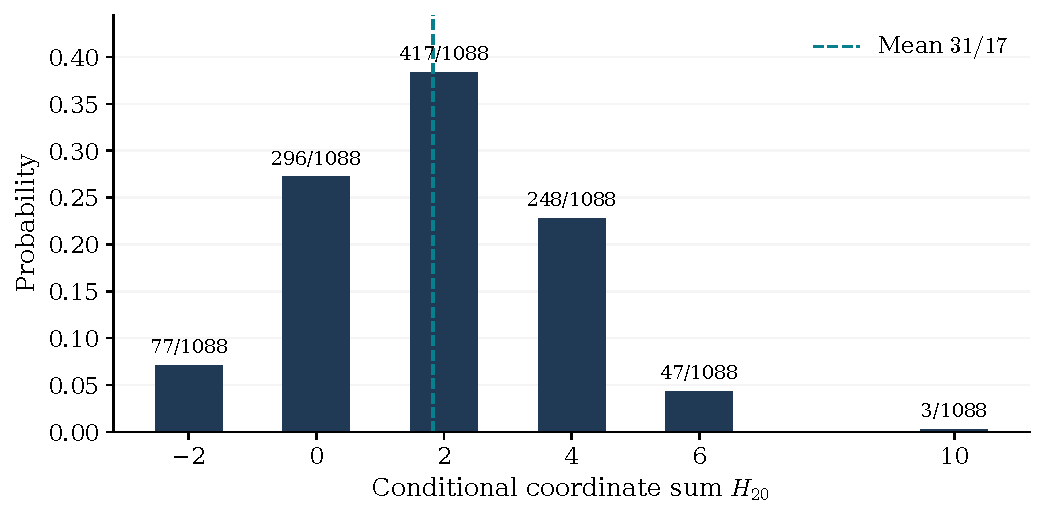
\includegraphics[width=.86\linewidth]{figures/exceptional_cell.pdf}
\caption{The exact conditional law on the exceptional twenty-bit cell.
The distribution is a law on six sums, with unequal spacings. Its
variance is \(1147/289<4\). The discrete probabilities, not a fitted
curve, determine the certificate.}
\label{fig:exceptional}
\end{figure}

Together with the codimension obstruction, Theorem~\ref{thm:witness}
proves Theorem~\ref{thm:headline}. It also shows why testing only
coordinate-subcube partitions would miss the phenomenon.

\subsection{The complete score law and its moments}

The four central values with mismatch \(-2\) have total ratio
\(77/12\); the remaining value has ratio \(1/4\).
Equation~\eqref{eq:finite-score-law} therefore simplifies to
\begin{equation}\label{eq:witness-score-law}
 \Law(T_{F_*})=\Law(H_{16})+
 \frac{-77\delta_2-3\delta_6+12\delta_4+68\delta_{31/17}}{8192}.
\end{equation}
This is a compact exact certificate for every score moment. For example,
\begin{align}
 \E T_{F_*}^3&=-\frac{6045}{591872},\notag\\
 \E T_{F_*}^4&=\frac{7403910529}{10061824}
             =736-\frac{1591935}{10061824},\label{eq:witness-moments}\\
 \kappa(F_*)&=\frac{15163208763392}{5275464041825}
             \simeq2.8742890944.\notag
\end{align}
Its moment generating function is the entire function
\begin{equation}\label{eq:witness-mgf}
 \E e^{tT_{F_*}}
 =(\cosh t)^{16}+
 \frac{-77e^{2t}-3e^{6t}+12e^{4t}+68e^{31t/17}}{8192}.
\end{equation}

\begin{lemma}[Symmetrizing an observation]\label{lem:symmetrize}
Let \(F\) be an observation of \(N\) bits with score \(T\), degree
\(D\), and variance \(v\). Introduce an independent sign \(z\), put
\(x'=zx\) coordinatewise, and report
\[
 F^{\mathrm{sym}}(z,x)=(z,F(x')).
\]
This is an observation of \(N+1\) bits with cell degree at most \(D+1\).
Its score is \(z(1+T)\), where \(z\) and \(T\) are independent, so
its law is symmetric and its retained variance is \(v+1\).
\end{lemma}

\begin{proof}
The change of variables \((z,x)\mapsto(z,x')\) preserves the uniform
product law. The full coordinate sum becomes \(z(1+H_N(x'))\);
conditioning gives the displayed score.
For each Walsh monomial in a cell indicator,
substitution produces \(z^{|S|}\chi_S(x)\).
Multiplication by \(\1_{\{z=\varepsilon\}}=(1+\varepsilon z)/2\)
has degree at most \(|S|+1\), proving the bound. Finally
\(\E(1+T)^2=1+v\).
\end{proof}

For our witness the symmetrized score has moment generating function
\[
 (\cosh t)^{17}
 +\frac{-77\cosh(3t)-3\cosh(7t)
       +12\cosh(5t)+68\cosh(48t/17)}{8192}.
\]
Its variance is \(591881/34816\) and its fourth moment is
\(8379512003/10061824\). Yet its first absolute moment is exactly
the seventeen-bit majority benchmark:
\begin{equation}\label{eq:oddified-benchmark}
 \E|z(1+T_{F_*})|=B_{17}.
\end{equation}
Indeed the correction to the first absolute moment is
\[
 \frac{-77\cdot3-3\cdot7+12\cdot5+68(48/17)}{8192}=0,
\]
and \(\E|1+H_{16}|=\E|H_{17}|\) by symmetry.
Likewise the correction to \(\E|T_{F_*}|\) in
\eqref{eq:witness-score-law} is zero, giving \(B_{16}\).
The exact degree of \(f=\sgn(T_{F_*})\) is 16. One certificate is
the coefficient \(165/16384\) on the set consisting of all four
central coordinates and all coordinates of leaf blocks 2, 3, and 4;
the verification script computes it by integer summation.
All possible scores are even integers or \(31/17\), so
\(\sgn(1+T_{F_*})=\sgn(T_{F_*})\). The symmetrized readout is therefore
\(z f(zx)\). The same nonzero degree-16 coefficient becomes a
degree-17 coefficient after multiplication by \(z\), proving its
exact degree is 17.
Thus these particular readouts have singleton sums \(B_{16}<\sqrt{16}\)
and \(B_{17}<\sqrt{17}\), respectively. The finite variance advantage
does not itself give a Boolean square-root counterexample.

\subsection{Tensorization, padding, and an extremal function}

\begin{definition}
For integers \(0\le D\le N\), let
\[
 V(N,D)=\max\{v(F):F\text{ is an observation of }N\text{ bits},
                  \ D(F)\le D\}.
\]
The maximum exists because a finite set has only finitely many
partitions; labels do not affect the value.
\end{definition}

\begin{theorem}[A global exact lower bound]\label{thm:tensor}
Put
\[
 q=\min\left\{\left\lfloor\frac D{16}\right\rfloor,
               \left\lfloor\frac{N-D}{4}\right\rfloor\right\}.
\]
Then
\begin{equation}\label{eq:extremal-lower}
 V(N,D)\ge D+\frac9{34816}q.
\end{equation}
If \(N-D\in\{0,1,2,3\}\), then \(V(N,D)=D\).
For every \(k\ge4\) and \(N\ge k+16\), there is an observation
of exact degree \(N-k\) with retained variance
\(N-k+9/34816\).
\end{theorem}

\begin{proof}
Take \(q\) disjoint copies of \(F_*\), reveal a further
\(r=D-16q\) individual signs, and ignore
\(s=N-D-4q\) signs. Both \(r\) and \(s\) are nonnegative integers,
and \(20q+r+s=N\). Lemma~\ref{lem:observation-calculus} gives exact
degree \(16q+r=D\) and variance
\(q(16+9/34816)+r\).
This proves \eqref{eq:extremal-lower}.
For deficits one through three the matching upper bound is the
codimension theorem; deficit zero uses \(v(F)\le N\).
For the final assertion use one copy, \(N-k-16\) revealed signs,
and \(k-4\) ignored signs.
\end{proof}

In particular, for \(q\ge1\),
\[
 V(20q,16q)\ge16q\left(1+\frac9{557056}\right).
\]
Thus no constant \(C\) can make \(v(F)\le D(F)+C\) hold for all
observations. At the single-cell level, the product cell \(A^q\) has
degree \(16q\) and conditional variance
\(4q-9q/289\). Tensorization makes the additive defect unbounded,
but leaves the ratio from this fixed witness unchanged. Improving
that ratio without bound requires a further mechanism, such as the
uniform amplifier below.

\begin{corollary}[A strict bound at codimension four]
\label{cor:strict-four}
For \(N\ge4\), every nonempty cell with
\(\deg\1_C\le N-4\) satisfies \(\Var(H_N\mid C)>3\).
Consequently
\[
 V(N,N-4)<N-3.
\]
\end{corollary}

\begin{proof}
The degree assumption gives the four alternating cancellations for
\(Y=(N-H_N)/2\). Proposition~\ref{codim:four-relaxation}
gives \(\Var(Y)>3/4\), proving the cellwise assertion.
Its positive-weight average gives \(v(F)<N-3\).
There are finitely many partitions of the \(N\)-cube, so the
maximum defining \(V(N,N-4)\) also satisfies the strict inequality.
\end{proof}

\subsection{An asymptotic retention profile}

\begin{proposition}[Existence and concavity of the profile]
\label{prop:profile}
For every \(0\le\rho\le1\), the limit
\[
 \Phi(\rho)=\lim_{N\to\infty}
        \frac{V(N,\lfloor\rho N\rfloor)}N
 =\sup_{N\ge1}\frac{V(N,\lfloor\rho N\rfloor)}N
\]
exists. The function is nondecreasing and concave, with
\(\Phi(0)=0\), \(\Phi(1)=1\), and
\begin{equation}\label{eq:profile-lower}
 \Phi(\rho)\ge\rho+\frac9{34816}
       \min\left\{\frac{\rho}{16},\frac{1-\rho}{4}\right\}.
\end{equation}
In particular \(\Phi(\rho)>\rho\) for every \(0<\rho<1\).
\end{proposition}

\begin{proof}
Tensorization gives
\[
 V(N_1+N_2,D_1+D_2)\ge V(N_1,D_1)+V(N_2,D_2).
\]
The degree budget is monotone, and
\(\lfloor\rho N_1\rfloor+\lfloor\rho N_2\rfloor
\le\lfloor\rho(N_1+N_2)\rfloor\).
Thus \(a_N=V(N,\lfloor\rho N\rfloor)\) is superadditive and
bounded above by \(N\). For completeness, fix \(r\) and write
\(N=qr+s\), \(0\le s<r\). Superadditivity and nonnegativity give
\(a_N\ge q a_r\); therefore
\(\liminf_Na_N/N\ge a_r/r\). Taking the supremum over \(r\)
proves existence and the displayed supremum formula.

Monotonicity follows directly from the degree budget. For concavity,
let \(\rho_1\ge\rho_2\), \(0<t<1\), and
\(\rho=t\rho_1+(1-t)\rho_2\).
Set \(N_1=\lfloor tN\rfloor\), \(N_2=N-N_1\). Then
\[
 \lfloor\rho_1N_1\rfloor+\lfloor\rho_2N_2\rfloor
 \le\left\lfloor\rho_2N+(\rho_1-\rho_2)N_1\right\rfloor
 \le\lfloor\rho N\rfloor.
\]
The product lower bound, divided by \(N\) and passed to the limit,
proves
\(\Phi(\rho)\ge t\Phi(\rho_1)+(1-t)\Phi(\rho_2)\).
The endpoint values follow from constant observations and full
revelation. Finally divide \eqref{eq:extremal-lower} by \(N\)
with \(D=\lfloor\rho N\rfloor\), and pass to the limit.
\end{proof}

\section{Exact minimality in a specified reporter family}
\label{enum:section}

The twenty-bit construction is small enough to admit a finite
minimality question. This section answers that question for the
binomial-block reporters defined below. It does not establish a
minimum dimension among all observations of a Boolean cube.

\subsection{The class being classified}

\begin{definition}[Binomial sum-level reporter]\label{enum:definition}
Choose positive integers \(n,m\), and take \(m+1\) independent blocks
of \(n\) uniform signs. Write their raw sums as
\(U,Z_1,\ldots,Z_m\). Their common alphabet and probabilities are
\[
 \mathcal S_n=\{x_j=2j-n:0\le j\le n\},\qquad
 p_j=2^{-n}\binom nj.
\]
Choose tests \(I_i\subseteq\mathcal S_n\) and a selector
\(\iota:\mathcal S_n\to[m]\), and use the refined report of
Section~\ref{sec:reporter}. In particular, an all-pass report reveals
all leaf sums, and an ordinary report reveals the central sum and all
unselected leaf sums. The total number of input bits is
\(N=n(m+1)\).
\end{definition}

The tests are unions of complete sum levels. They cannot distinguish
two sign strings having the same sum. This restriction is part of the
definition and part of the minimality conclusion.

\begin{lemma}[Exact degree of a nonconstant reporter]
\label{enum:exact-degree}
Every nonconstant reporter in Definition~\ref{enum:definition} has
maximum cell degree exactly \(nm\).
\end{lemma}

\begin{proof}
Proposition~\ref{prop:reporter} gives the upper bound. The indicator
of any nonempty \(n\)-bit sum level has degree exactly \(n\): its
top Walsh character is constant, with value
\((-1)^{(n-x_j)/2}\), throughout that level, so the corresponding
coefficient is that sign times \(p_j\), and is nonzero.

If all tests are nonempty, choose one allowed value in each test.
The corresponding all-pass cell fixes these \(m\) raw leaf sums and
places no condition on the center. Its indicator is a product of
\(m\) level indicators on disjoint blocks. Their nonzero top
coefficients multiply, giving degree \(nm\).

If a test is empty, the all-pass event is empty. Unless the whole
observation is the single exceptional tag, there is an attained
ordinary cell. Such a cell fixes the central sum and \(m-1\)
unselected leaf sums; its reported values already force an unselected
failure. Its indicator is again a product of \(m\) level indicators,
and has degree \(nm\).
\end{proof}

Thus an advantage over the block bound \(nm\) is an advantage over
the actual maximum cell degree, apart from constant observations,
which have no advantage.

\subsection{The exact finite objective}

The singleton formula of Theorem~\ref{thm:finite-selector} extends
to arbitrary nonempty proper tests without numerical integration.
For test \(I_i\), put
\[
 \beta_i=\Pbb(Z_i\in I_i),\quad
 \mu_i=\E[Z_i\mid Z_i\in I_i],\quad
 s_i^2=\Var(Z_i\mid Z_i\in I_i).
\]
For a selector \(j\mapsto i_j=\iota(x_j)\), define
\begin{align*}
 Q&=\prod_i\beta_i,& S&=\sum_i s_i^2,&
 w_j&=p_j/\beta_{i_j},\\
 R_0&=\sum_jw_j,& K&=R_0-1,&
 R_1&=\sum_jw_j(x_j-\mu_{i_j}),\\
 H_2&=\sum_jw_j(x_j-\mu_{i_j})^2.&&&&
\end{align*}
Every number here is rational. Since all tests are proper,
\(\beta_i<1\), and hence \(K>0\).

\begin{proposition}[Objective for arbitrary sum-level tests]
\label{enum:objective}
For the reporter \(F\), its exact advantage is
\begin{equation}\label{enum:gain}
 g:=v(F)-nm
 =Q\left\{\frac{R_1^2}{K}-H_2-KS+
               \sum_j w_j s_{i_j}^2\right\}.
\end{equation}
The exceptional cell has probability \(QK\) and optimal predictor
\[
 b_* = \sum_i\mu_i+\frac{R_1}{K}.
\]
\end{proposition}

\begin{proof}
The identities \(\Pbb(P)=QR_0\), \(\Pbb(B)=Q\), and
\(\Pbb(A)=QK\) follow by conditioning on the center.
For a constant exceptional predictor \(b\), put
\(C=\sum_i\mu_i-b\). Conditional on \(U=x_j\) and \(P\), the
mean of \(L-b\) is \(x_j+C-\mu_{i_j}\), and its variance is
\(n+S-s_{i_j}^2\). On \(B\), its mean is \(C\) and its variance
is \(n+S\). Subtracting the contribution of \(B\) from that of
\(P\) gives
\[
 \E[\1_A\{n-(L-b)^2\}]
 =Q\left\{-KC^2-2R_1C-H_2-KS+
                       \sum_jw_js_{i_j}^2\right\}.
\]
The maximum occurs at \(C=-R_1/K\). The optimizing predictor is
the conditional mean on \(A\), so
\eqref{eq:optimal-exceptional} identifies the maximum with
\(v(F)-nm\). This proves \eqref{enum:gain}.
\end{proof}

\subsection{Reductions that make the enumeration complete}

\begin{lemma}[Reduction to distinct proper tests and onto selectors]
\label{enum:reductions}
If a reporter has positive advantage, then it has no empty or full
leaf test. From any positive reporter one can obtain another positive
reporter with no more input bits, distinct tests, and a surjective
selector. A reporter with one leaf has no positive advantage.
\end{lemma}

\begin{proof}
If at least two tests are empty, \(A\) is empty. If exactly one test,
at leaf \(i\), is empty, then \(A\) requires selecting \(i\) and
the success of all other tests. Thus \(A\) is independent of
\(Z_i\), which retains variance \(n\) on that event. In either
case \eqref{eq:optimal-exceptional} rules out a positive advantage.

If test \(i\) is full, then \(A\) is false when \(i\) is selected,
and is independent of \(Z_i\) when another leaf is selected.
Consequently \(A\) is independent of \(Z_i\) altogether. Again
\(\Var(L\mid A)\ge n\), whenever \(A\) is nonempty. This also
rules out using a full test as a favorable selector fallback.

Suppose next that a proper nonempty leaf test is never selected.
Deleting it leaves \(K,R_1,H_2\) and the selected-variance term in
\eqref{enum:gain} unchanged, decreases \(S\) by \(s_i^2\), and
divides \(Q\) by \(\beta_i\). The new advantage is
\[
 g'=\frac{g}{\beta_i}+\frac{QK}{\beta_i}s_i^2>0.
\]
If two tests coincide, merge their selector labels. The parameters
in \eqref{enum:gain} do not change, because the two tests have the
same probability, mean, and variance. One copy is now unused and
can be deleted. Repeating these operations gives the stated
reduction. A surjective selector has at most \(n+1\) leaf labels.

Finally, when \(m=1\), the reporter only describes its leaf and
never the independent center. Its retained variance is at most
\(n\). By Lemma~\ref{enum:exact-degree}, a nonconstant such
reporter has degree \(n\); a constant one has both variance and
degree zero.
\end{proof}

\subsection{The finite certificate}

\begin{theorem}[Twenty-bit minimality in the binomial reporter class]
\label{enum:minimality}
No reporter in Definition~\ref{enum:definition} on fewer than twenty
bits has retained variance greater than its maximum cell degree.
The reporter of Theorem~\ref{thm:witness} attains a strict advantage
on twenty bits. Thus twenty is the minimum within this specified
class.
\end{theorem}

\begin{proof}
It suffices to consider a nonconstant reporter with distinct nonempty
proper tests and a surjective selector, by
Lemmas~\ref{enum:exact-degree} and~\ref{enum:reductions}.
Its codimension is exactly \(n\). If \(n\le3\), the analytic
codimension obstruction excludes an advantage. The case \(m=1\)
has already been excluded. If \(n\ge7\) and \(m\ge2\), then
\(n(m+1)\ge21\). Therefore fewer than twenty bits leave only the
four parameter pairs in the following table.

\begin{center}
\begin{tabular}{@{}rrrrr@{}}
\toprule
Block size \(n\)&Leaves \(m\)&Bits \(N\)&Configurations&Maximum \(g\)\\
\midrule
4&2&12&13,050&\(-1/12\)\\
4&3&16&609,000&\(-35/17152\)\\
5&2&15&117,242&\(-595/8576\)\\
6&2&18&992,250&\(-1293/33152\)\\
\bottomrule
\end{tabular}
\end{center}

There are \(q_n=2^{n+1}-2\) nonempty proper sum-level tests. The
certificate enumerates every unordered family of \(m\) distinct
tests and every onto map from the \(n+1\) central sums to those
tests. The exact number of configurations is therefore
\begin{equation}\label{enum:count}
 \binom{q_n}{m}
 \sum_{r=0}^m(-1)^r\binom mr(m-r)^{n+1}.
\end{equation}
This gives exactly the counts in the table. Sorting the test masks
only removes permutations of leaf labels; all selectors for each
sorted family are still included.

The program \texttt{code/enumerate\_reporters.py} evaluates
\eqref{enum:gain} with integer fractions for every configuration,
compares them exactly, and obtains the displayed maxima. All
1,731,542 configurations have nonpositive advantage; in these four
reduced cases the maxima are strictly negative. The JSON output
records the counts and a maximizing family, selector, and predictor
for each row. This exact finite exhaustion completes the lower
bound. The twenty-bit upper bound is
Theorem~\ref{thm:witness}.
\end{proof}

The only computational part of this theorem is the four-row finite
exhaustion. The codimension threshold and the positive twenty-bit
construction have independent mathematical proofs. In particular,
their validity does not depend on this minimality search.

\subsection{Reproduction and limits of the certificate}

The companion code uses only the Python standard library. The command
\begin{verbatim}
python code/run_verification.py
\end{verbatim}
checks the twenty-bit witness and writes
\texttt{data/witness\_certificate.json}. It enumerates all \(5^5=3125\)
tuples of block sums, with their exact binomial multiplicities, so
every one of the \(2^{20}\) sign strings is accounted for. All 622
cells, their conditional moments, the complete score law, and the
retained variance are checked.

The same verifier also performs a complete degree check. Block symmetry
makes a Walsh coefficient depend only on the five subset sizes in its
blocks. There are 56 such profiles of total degree greater than 16;
all their coefficients vanish on each of the 622 cells, giving 34,832
exact zero checks. A degree-16 coefficient is nonzero on every cell.
The code uses the exact sum of a fixed character on each binomial
layer, rather than a numerical transform.

To regenerate the complete minimality certificate, run
\begin{verbatim}
python code/run_verification.py --exhaustive
\end{verbatim}
This writes \nolinkurl{data/minimality_certificate.json}. A separate
implementation, \nolinkurl{code/enumerate_two_leaf_integer.py},
uses cross-multiplied integer comparisons in its inner loop. The
included independent check of the largest two-leaf case agrees with
the fraction implementation on all 992,250 configurations and on
the exact maximum \(-1293/33152\).

These are reproducible finite certificates, not a Lean formalization
of the enumeration programs. They do not exclude smaller witnesses
outside Definition~\ref{enum:definition}, including leaf tests that
split individual sum levels, unequal block sizes, different reporting
mechanisms, or general partitions of a cube.

\section{A uniform quantitative amplification theorem}
\label{amp:sec}

The amplification argument of \cite{OpenAI2026} takes a sufficiently large
finite average separately at each stage.  We now give conditions under which
one averaging count works at every stage, together with explicit bounds for
that count.  The main point is to control the error relative to the product
of the interval probabilities.  The product itself will not enter the required
normal-approximation accuracy.  Positive-power growth can also be obtained
nonquantitatively from a Boolean seed by the composition argument in
Section~\ref{subsec:composition}; the result here supplies fixed
parameters and dimension bounds.

For a finite observation $F$ of $N$ independent fair signs, retain the notation
\[
 H_N=\sum_{i=1}^N X_i,\qquad T_F=\E[H_N\mid F],\qquad
 v(F)=\E T_F^2.
\]
When $v(F)>0$, write
\[
 \kappa(F)=\frac{\E T_F^4}{v(F)^2}.
\]
All degree bounds in this section are bounds on the indicators of the
attained cells.  A function of an observation then has the same degree bound.

\subsection{The reporting identity for nonsingleton intervals}

We restate the reporting construction of \cite{OpenAI2026} in the form
needed for quantitative estimates.  Fix $m\ge3$, bounded intervals
$I_1,\ldots,I_m$, a selector $\iota:\R\to\{1,\ldots,m\}$, and a real
number $c$.  Apply the rule to independent copies
$(U,Z_1,\ldots,Z_m)$ of a centered variance-one random variable.  Put
\[
 L_0=U+\sum_{j=1}^m Z_j,\qquad
 \mathsf B=\bigcap_j\{Z_j\in I_j\},\qquad
 \mathsf P=\bigcap_{j\ne\iota(U)}\{Z_j\in I_j\},\qquad
 \mathsf A=\mathsf P\setminus\mathsf B.
\]
The observation $\mathcal W$ reports the tag $\mathsf A$ on $\mathsf A$,
the tag $\mathsf B$ and all leaf values on $\mathsf B$, and the tag
$\mathsf P^c$, the central value, the selected index, and all unselected
leaf values on $\mathsf P^c$.  The identity
\begin{equation}
 \1_{\mathsf A}
 =\sum_{i=1}^m\1_{\{\iota(U)=i\}}
                 \prod_{j\ne i}\1_{I_j}(Z_j)
       -\prod_{j=1}^m\1_{I_j}(Z_j)
 \label{amp:cell-identity}
\end{equation}
shows that every cell indicator is a linear combination of functions of at
most $m$ input coordinates.  For an ordinary report on $\mathsf P^c$, the
reported leaves already certify a failed test, so the omitted leaf is
unrestricted.  This verifies the same assertion for all ordinary reports,
including on finite alphabets with atoms at interval endpoints.

For a centered variance-one law $V$, define
\begin{align}
 q_i^V&=\Pbb(V\in I_i),&
 \mu_i^V&=\E[V\mid V\in I_i],\notag\\
 s_i^V&=\Var(V\mid V\in I_i),&
 Q_V&=\prod_iq_i^V,\quad S_V=\sum_i s_i^V,
 \label{amp:interval-parameters}
\end{align}
whenever all $q_i^V$ are positive.  Thus $s_i^V$ denotes a variance, not
a standard deviation.  With $C_i=\{t:\iota(t)=i\}$, put
\begin{equation}
 J_V=\sum_{i=1}^m\frac1{q_i^V}
       \E\left[\1_{C_i}(V)
       \left((V+c-\mu_i^V)^2+\sum_{j\ne i}s_j^V\right)\right].
 \label{amp:J}
\end{equation}

\begin{proposition}[Exact predictor gain]
\label{amp:reporter}
For the reporting rule above, use the predictor
$b_V=\sum_i\mu_i^V-c$ on $\mathsf A$, the sum of the leaves on
$\mathsf B$, and the sum of the reported values on $\mathsf P^c$.
Its mean squared error is
\begin{equation}
 1-\Delta_V,\qquad
 \Delta_V=Q_V(c^2+S_V-J_V).
 \label{amp:relative-gain}
\end{equation}
Consequently
\begin{equation}
 \Var\bigl(\E[L_0\mid\mathcal W]\bigr)\ge m+\Delta_V.
 \label{amp:variance-gain}
\end{equation}
On every product of finite input alphabets, the observation has finite
range and the coordinate-degree property stated after
\eqref{amp:cell-identity}.
\end{proposition}

\begin{proof}
The error on $\mathsf B$ is the unreported central input.  The error on
each ordinary report is its unreported leaf.  Independence therefore makes
the integrated squared errors on these events equal to their probabilities.
It follows that the total error is
$1-\E[\1_{\mathsf A}(1-(L_0-b_V)^2)]$.

Conditional on $U=t$ and $\mathsf P$, the event has probability
$Q_V/q_{\iota(t)}^V$, and $L_0-b_V$ has mean
$t+c-\mu_{\iota(t)}^V$ and variance
$1+\sum_{j\ne\iota(t)}s_j^V$.  Thus the contribution on
$\mathsf P$ to the last gain is $-Q_VJ_V$.  On $\mathsf B$, the
central input remains unrestricted; the same difference has mean $c$ and
variance $1+S_V$.  Its contribution is $-Q_V(c^2+S_V)$.
Subtracting, since $\1_{\mathsf A}=\1_{\mathsf P}-\1_{\mathsf B}$,
proves \eqref{amp:relative-gain}.  Conditional expectation minimizes
mean squared error, and $\Var(L_0)=m+1$, proving
\eqref{amp:variance-gain}.  The finite-alphabet assertion follows from
\eqref{amp:cell-identity} and the description of the ordinary reports.
\end{proof}

The law-dependent predictor $b_V$ is only a tool for estimating the error.
The observation $\mathcal W$, its cells, and their degree bounds do not
depend on $b_V$.

\subsection{Restricted moments from a Kolmogorov bound}

Write $d_{\mathrm K}$ for Kolmogorov distance and let $G$ denote a standard
normal random variable.

\begin{lemma}[Restricted first and second moments]
\label{amp:restricted}
Suppose $U$ is centered, has variance one, and satisfies $\E U^4\le K$,
where $K\ge3$.  If $d_{\mathrm K}(U,G)\le\delta\le1$ and $E$ is a
union of at most $\ell$ intervals, then
\begin{align}
 |\Pbb(U\in E)-\Pbb(G\in E)|&\le2\ell\delta,\\
 |\E[U\1_E(U)]-\E[G\1_E(G)]|
   &\le(2\ell+3)K^{1/4}\delta^{3/4},\\
 |\E[U^2\1_E(U)]-\E[G^2\1_E(G)]|
   &\le(2\ell+4)\sqrt{K\delta}.
 \label{amp:restricted-bounds}
\end{align}
Unbounded intervals and arbitrary endpoint conventions are allowed.
For one bounded interval $I\subseteq[-B,B]$, the unnormalized moments
also satisfy the sharper estimates
\begin{equation}
 \begin{aligned}
 |q_U-q_G|&\le2\delta,\\
 |\E[U\1_I(U)]-\E[G\1_I(G)]|&\le4B\delta,\\
 |\E[U^2\1_I(U)]-\E[G^2\1_I(G)]|&\le4B^2\delta.
 \end{aligned}
 \label{amp:bounded-moments}
\end{equation}
\end{lemma}

\begin{proof}
Let $D(t)=F_U(t)-\Phi_{\mathrm G}(t)$, where $\Phi_{\mathrm G}$ is
the standard normal distribution function. Both fourth moments are at most $K$.
Markov's inequality, applied to the appropriate right or left tail, gives
\[
 |D(t)|\le\min\{\delta,K/|t|^4\}.
\]
The same bound holds at left limits.  If $\delta>0$, split the following
integrals at $R=(K/\delta)^{1/4}$ to obtain
\begin{equation}
 \int_{\R}|D(t)|\,dt\le\frac83K^{1/4}\delta^{3/4},\qquad
 \int_{\R}2|tD(t)|\,dt\le4\sqrt{K\delta}.
 \label{amp:cdf-integrals}
\end{equation}
At any endpoint, $|tD(t)|\le K^{1/4}\delta^{3/4}$ and
$|t^2D(t)|\le\sqrt{K\delta}$.  Stieltjes integration by parts over
the disjoint intervals now gives the first assertion.  There are at most
$2\ell$ finite endpoint contributions; the integral terms in
\eqref{amp:cdf-integrals} need be counted only once.  The constants
$2\ell+3$ and $2\ell+4$ follow.  Boundary terms at infinity vanish
by the fourth-moment bound.  Left limits handle any atoms at an included
or excluded endpoint.  When $\delta=0$, the laws coincide.

For a bounded interval, the total variations of its indicator, of $t$
times its indicator, and of $t^2$ times its indicator are bounded by
$2$, $4B$, and $4B^2$, respectively.  The same integration-by-parts
argument gives \eqref{amp:bounded-moments}.
\end{proof}

\subsection{Transfer of a fixed Gaussian gain}

\begin{theorem}[Explicit relative transfer]
\label{amp:transfer}
Assume $I_i\subseteq[-B,B]$ with $B\ge1$, and each selector cell $C_i$
is a union of at most $\ell$ intervals.  In the Gaussian model, suppose
\[
 q=\min_i q_i^G>0,\qquad
 \Gamma=c^2+S_G-J_G>0.
\]
For $K\ge3$, set $C=|c|+B$ and
\begin{align}
 A={}&\frac{36mB^2}{q}\notag\\
 &+\frac{2m}{q}\left((2\ell+4)\sqrt K
      +2C(2\ell+3)K^{1/4}+2\ell(C^2+mB^2)\right)\notag\\
 &+\frac{48B(1+C)+76mB^2+4(1+C)^2}{q^2},
 \label{amp:A}\\
 \delta_*={}&\min\left\{1,\frac{q}{4m},
                           \left(\frac{\Gamma}{2A}\right)^2\right\}.
 \label{amp:delta-star}
\end{align}
Every centered variance-one law $U$ with $\E U^4\le K$ and
$d_{\mathrm K}(U,G)\le\delta_*$ satisfies
\begin{equation}
 Q_U\ge Q_G/2,\qquad c^2+S_U-J_U\ge\Gamma/2,\qquad
 \Delta_U\ge Q_G\Gamma/4.
 \label{amp:transfer-conclusion}
\end{equation}
\end{theorem}

\begin{proof}
Write $\delta=d_{\mathrm K}(U,G)$.  Since $\delta\le q/(4m)$,
all interval probabilities for $U$ are positive.  The bounded-interval
estimates in Lemma~\ref{amp:restricted} imply
\begin{align}
 |\mu_i^U-\mu_i^G|&\le\frac{12B\delta}{q},&
 |s_i^U-s_i^G|&\le\frac{36B^2\delta}{q},\\
 \left|\frac1{q_i^U}-\frac1{q_i^G}\right|&\le\frac{4\delta}{q^2},&
 \frac1{q_i^U}&\le\frac2q.
 \label{amp:parameter-errors}
\end{align}
For example, the first conditional moment changes by at most
$(4B\delta+2B\delta)/(q/2)=12B\delta/q$.  The conditional
second moment changes by at most $12B^2\delta/q$; subtracting the
squared means costs at most a further $24B^2\delta/q$.
Moreover,
\[
 \frac{Q_U}{Q_G}
 \ge\prod_i\left(1-\frac{2\delta}{q_i^G}\right)
 \ge1-\frac{2m\delta}{q}\ge\frac12.
\]

For completeness, we bound $J_U-J_G$ with all factors displayed.
Put
\[
 N_i^V(t)=(t+c-\mu_i^V)^2+\sum_{j\ne i}s_j^V.
\]
In \eqref{amp:J}, first replace $N_i^U$ by $N_i^G$ under the law
of $U$, then replace that law by the Gaussian law, and finally replace
$1/q_i^U$ by $1/q_i^G$.  The three absolute errors are at most,
respectively,
\begin{align}
 E_1&=\frac{\delta}{q^2}
                 \left(48B(1+C)+72mB^2\right),\\
 E_2&=\frac{2m}{q}\Bigl((2\ell+4)\sqrt{K\delta}
       +2C(2\ell+3)K^{1/4}\delta^{3/4}\notag\\
    &\hspace{37mm}+2\ell(C^2+mB^2)\delta\Bigr),\\
 E_3&=\frac{4\delta}{q^2}\left((1+C)^2+mB^2\right).
 \label{amp:three-errors}
\end{align}
For $E_1$, use
\[
 |(t+c-\mu_i^U)^2-(t+c-\mu_i^G)^2|
 \le\frac{24B\delta}{q}(|t|+C),
\]
together with \eqref{amp:parameter-errors}.  The cells $C_i$ partition
the line and $\E|U|\le1$, so these terms are summed before taking
expectations.  For $E_2$, expand the fixed quadratic $N_i^G$ and use
\eqref{amp:restricted-bounds}; its three coefficient bounds are
$1$, $2C$, and $C^2+mB^2$.  For $E_3$, use the denominator estimate
and $\E|G|\le1$, again summing over the partition first.

Finally $|S_U-S_G|\le36mB^2\delta/q$.  Since
$\delta\le1$, equations \eqref{amp:A} and \eqref{amp:three-errors}
give
\[
 |S_U-S_G|+|J_U-J_G|\le A\sqrt\delta\le\Gamma/2.
\]
Together with the product bound, this proves
\eqref{amp:transfer-conclusion}.
\end{proof}

The hypotheses are fixed one-dimensional estimates.  In particular,
$\delta_*$ depends on $q$, $\Gamma$, the number of leaves, and the
geometry of the intervals, while the small product $Q_G$ determines
the eventual gain rather than the accuracy requirement.

\subsection{One averaging count for every stage}

\begin{theorem}[Fixed-count amplification]
\label{amp:fixed-count}
Assume the hypotheses of Theorem~\ref{amp:transfer}, use $K=6$, and
choose an integer
\[
 M\ge\max\{2,\lceil6/\delta_*^2\rceil\}.
\]
Let $0<\eta\le Q_G\Gamma/4$, and set
\begin{equation}
 \begin{aligned}
 d_*&=mM,\qquad n_*=(m+1)M,\qquad v_*=M(m+\eta),\\
 \alpha&=\frac{\log v_*}{2\log d_*}
       =\frac12+\frac{\log(1+\eta/m)}{2\log(mM)}.
 \end{aligned}
 \label{amp:scales}
\end{equation}
Writing $L(f)=\sum_i\widehat f(\{i\})$, there are finite observations
$F_k$ and Boolean readouts $f_k$ such that
\begin{align}
 N_k&=n_*^k,& \degc(F_k)&\le d_*^k,\notag\\
 v(F_k)&\ge v_*^k,& \kappa(F_k)&\le6,\notag\\
 \deg(f_k)&\le d_*^k,& L(f_k)&\ge6^{-1/2}d_*^{k\alpha}.
 \label{amp:iterates}
\end{align}
In particular, the Boolean degrees tend to infinity and
$L(f_k)\ge6^{-1/2}\deg(f_k)^\alpha$.
\end{theorem}

\begin{proof}
For a finite observation with score $T$, positive variance $v$, and
$\E T^4/v^2\le6$, take $M$ independent copies and form
\[
 Z=\frac{T_1+\cdots+T_M}{\sqrt{Mv}}.
\]
Its score as an observation of the underlying signs is exactly
$\sqrt{Mv}\,Z$, and its cell degree is at most $M\degc(F)$.
Writing $\kappa=\E T^4/v^2$, independence gives
\begin{equation}
 \E Z^4=3+\frac{\kappa-3}{M}.
 \label{amp:average-fourth}
\end{equation}
The Berry--Esseen inequality with an absolute constant below one
\cite{Shevtsova2011}, and
$\E|T/\sqrt v|^3\le\sqrt\kappa$, give
\begin{equation}
 d_{\mathrm K}(Z,G)\le\sqrt{6/M}\le\delta_*.
 \label{amp:BE}
\end{equation}
Thus Theorem~\ref{amp:transfer} applies to $m+1$ independent copies
of $Z$.  If $F'$ is their report, the conditional-expectation identity
for the total underlying sign sum gives
\[
 v(F')\ge Mv(m+\eta),\qquad \degc(F')\le mM\degc(F).
\]

It remains to check the fourth moment uniformly.  Let $r=m+1$,
$S_0=Z_1+\cdots+Z_r$, and
$V=\Var(\E[S_0\mid F'])\ge m+\eta$.  Conditional Jensen's
inequality and independence yield
\begin{align}
 \kappa(F')\le\frac{\E S_0^4}{V^2}
 &\le\frac{3r^2+r(\kappa-3)/M}{(m+\eta)^2}\notag\\
 &\le\frac{3(m+1)^2+3(m+1)/2}{m^2}\le6.
 \label{amp:moment-invariant}
\end{align}
The last inequality follows from
\[
 6m^2-3(m+1)^2-\tfrac32(m+1)
 =\tfrac32(2m+1)(m-3)\ge0.
\]
Start with one revealed sign, whose variance and cell degree are both
one and whose standardized fourth moment is one.  Induction proves
the observation assertions in \eqref{amp:iterates} with the same $M$
at every step.

Take $f_k=\operatorname{sign}(T_{F_k})$, with sign $+1$ at zero.
It is a function of the observation, so has the stated degree bound,
and conditioning gives $L(f_k)=\E|T_{F_k}|$.
For any centered variance-one $Y$, H\"older's inequality gives
\[
 1=\E Y^2\le(\E|Y|)^{2/3}(\E Y^4)^{1/3}.
\]
Thus $\E|T_{F_k}|\ge\sqrt{v(F_k)/6}$, which proves the lower
bound.  Finally every Boolean function satisfies $L(f)\le\deg(f)$:
each absolute singleton coefficient is at most its influence, and the
sum of the influences is at most the degree by Parseval.  Hence the
degrees here tend to infinity.
\end{proof}

\begin{corollary}[Degree budgets and ambient dimension]
\label{amp:dimension}
With the notation of Theorem~\ref{amp:fixed-count}, put
\[
 \theta=\frac{\log n_*}{\log d_*},\qquad
 \beta=\frac{2\log n_*}{\log v_*}.
\]
For every real degree budget $D\ge d_*$, one of the readouts has
\begin{equation}
 \deg(f)\le D,\qquad n\le D^\theta,\qquad
 L(f)\ge6^{-1/2}d_*^{-\alpha}D^\alpha.
 \label{amp:budget}
\end{equation}
For each individual iterate, its actual degree $d=\deg(f_k)$ also gives
\begin{equation}
 N_k\le(\sqrt6\,d)^\beta.
 \label{amp:actual-degree}
\end{equation}
\end{corollary}

\begin{proof}
Choose $k=\lfloor\log D/\log d_*\rfloor$.  Then
$D/d_*<d_*^k\le D$, and \eqref{amp:budget} follows from
\eqref{amp:iterates}.  For \eqref{amp:actual-degree}, the already
proved inequality
$d\ge L(f_k)\ge6^{-1/2}v_*^{k/2}$ implies
$(\sqrt6\,d)^\beta\ge n_*^k=N_k$.
\end{proof}

If all interval endpoints and selector cut points are rational, these
constructions are terminating exact algorithms.  Every unnormalized score
and its variance are rational because the underlying cube is finite.  A
normalized score is a quadratic algebraic number, so comparisons with the
fixed rational cut points are decidable, including equality.  Conditional
scores can be obtained by finite enumeration of cells.  The dimension and
degree bounds quantify mathematical size; no efficient running-time claim
is made.

\section{A completely explicit rational Gaussian seed}
\label{gaussian:sec}

We now instantiate Section~\ref{amp:sec}.  The parameters are deliberately
conservative: their purpose is to give a reproducible numerical theorem
using rational inequalities, with no unspecified ``sufficiently large''
choice.  The resulting exponent is very small.  The construction complements
the small exact witness and the codimension classification rather than
providing a practical Boolean example.

\subsection{Intervals and selector}

Set
\begin{equation}
 \begin{aligned}
 s&=2^{13},\qquad m=s^2+1=2^{26}+1,\qquad R=9,\\
 c&=\frac13,\qquad h=\frac9{s^3}=\frac9{2^{39}}.
 \end{aligned}
 \label{gaussian:parameters}
\end{equation}
For $0\le i<m$, take
\begin{equation}
 a_i=c-9+\frac{18i}{m-1},\qquad I_i=[a_i-h,a_i+h].
 \label{gaussian:intervals}
\end{equation}
For $|t|\le9$, the selector chooses a center nearest to $t+c$, with
ties resolved by the smaller index.  For $|t|>9$, it chooses the middle
index, whose center is $c$.  Every endpoint and cut point is rational.
Each selector cell is an interval except for the middle cell, which is
a union of at most three intervals.  Thus $\ell=3$ is valid in
Theorem~\ref{amp:transfer}.

Let $q_i,\mu_i,s_i$ be the Gaussian interval probabilities, means, and
variances from \eqref{amp:interval-parameters}, and write
$Q=\prod_iq_i$, $S=\sum_i s_i$, and $J=J_G$.  Define
\[
 r_0=\frac9{s^2},\qquad e_0=r_0+h.
\]
The elementary interval estimates are
\begin{equation}
 |\mu_i-a_i|\le h,\qquad 0\le s_i\le h^2,\qquad
 S\le mh^2=\frac{81}{s^4}(1+s^{-2}).
 \label{gaussian:interval-estimates}
\end{equation}
On $|t|\le9$, nearest-center selection additionally gives
$|t+c-\mu_{\iota(t)}|\le e_0$.

\begin{lemma}[Certified Gaussian gain]
\label{gaussian:gain}
The parameters \eqref{gaussian:parameters}--\eqref{gaussian:intervals}
satisfy
\begin{equation}
 J_{\rm central}<\frac3{40},\qquad
 J_{\rm tail}<\frac1{1000},\qquad
 \Gamma:=c^2+S-J>\frac1{32}.
 \label{gaussian:gain-bounds}
\end{equation}
Moreover every interval is contained in $[-10,10]$, and
\begin{equation}
 q:=\min_iq_i>
 q_0:=\frac1{2^{38}3^{49}}>2^{-116}.
 \label{gaussian:q-bound}
\end{equation}
\end{lemma}

\begin{proof}
Write $\phi(t)=(2\pi)^{-1/2}e^{-t^2/2}$.  If $|t|\le9$ and
$z\in I_{\iota(t)}$, then $z-t=c+\xi$ with $|\xi|\le e_0$.
Consequently
\[
 \frac{z^2-t^2}{2}
 \le ct+\frac{c^2}{2}+e_0(9+c)+\frac{e_0^2}{2}
 <ct+\frac1{16}.
\]
The last inequality is a rational comparison after substituting
\eqref{gaussian:parameters}; it is also among the checks in the
constant certificate below.  Taking the minimum density on the selected
interval gives
\begin{equation}
 \frac{\phi(t)}{q_{\iota(t)}}
 \le\frac{e^{1/16}e^{ct}}{2h}
 \qquad(|t|\le9).
 \label{gaussian:density-ratio}
\end{equation}
Inserting \eqref{gaussian:interval-estimates} into
\eqref{amp:J} and integrating $e^{ct}$, we obtain
\begin{align}
 J_{\rm central}
 &\le\frac{3(e_0^2+mh^2)}{h}e^{1/16}\sinh3\notag\\
 &=\frac{54}{s}(1+s^{-1}+s^{-2})e^{1/16}\sinh3.
 \label{gaussian:central}
\end{align}
The elementary series bound $e^x<(1-x)^{-1}$ for $0<x<1$
gives $e^{1/16}<16/15$.  Also $e<11/4$ implies
$\sinh3<e^3/2<21/2$.  Thus the last expression is less than
\[
 \frac{54}{8192}(1+8192^{-1}+8192^{-2})\frac{16}{15}\frac{21}{2}
 <\frac3{40}.
\]
For an entirely rational justification of the bound on $e$, sum its
series through $1/3!$ and bound the remaining factorial tail by
$(1/24)\sum_{j\ge0}5^{-j}=5/96$.  This gives
$e<87/32<11/4$; the strict lower bound $e>5/2$ follows from the
first three terms and the positive remainder.

On $|t|>9$ the fallback interval has center $c$, and
$c+h<1/2$.  Its probability is at least $2h\phi(1/2)$.
Since $h<1$, $S<1$, and $|t|\ge9$,
\[
 (t+c-\mu_{\rm middle})^2+\sum_{j\ne\rm middle}s_j
 \le(|t|+h)^2+S\le2t^2.
\]
Integration by parts and the Gaussian tail bound give
\[
 \int_9^\infty t^2e^{-t^2/2}\,dt
 \le\left(9+\frac19\right)e^{-81/2}.
\]
Using both tails therefore yields
\begin{equation}
 J_{\rm tail}\le\frac{164}{9h}e^{-323/8}
 <\frac{55}{3h}e^{-323/8}
 <\frac{55\,2^{79}}{27\,5^{40}}
 <\frac1{1000}.
 \label{gaussian:tail}
\end{equation}
Here $323/8>40$ and $e>5/2$ justify the penultimate exponential
comparison.  In particular,
\[
 \Gamma\ge c^2-J
 >\frac19-\frac3{40}-\frac1{1000}
 =\frac{79}{2250}>\frac1{32}.
\]

Finally, $|a_i|+h<10$ for every $i$.  Since $\sqrt{2\pi}<3$,
\[
 q_i\ge2h\min_{z\in I_i}\phi(z)
 >\frac{2h}{3}e^{-50}
 >\frac{2h}{3}\,3^{-50}
 =\frac1{2^{38}3^{49}}.
\]
The last strict inequality uses $e<3$.  The integer inequality
$3^{49}<2^{78}$ now proves \eqref{gaussian:q-bound}.
\end{proof}

\subsection{A fixed averaging count and an explicit exponent}

\begin{theorem}[Fully numerical quantitative instance]
\label{gaussian:explicit}
For the rational reporting rule above, set
\begin{equation}
 M=2^{1123},\qquad
 \eta_0=2^{-(116m+7)},\qquad
 \varepsilon_0=2^{-8\,000\,000\,000}.
 \label{gaussian:numerical-choices}
\end{equation}
There is a sequence of exactly specified finite Boolean functions $f_k$
on $((m+1)M)^k$ bits, with
\begin{equation}
 \begin{aligned}
 \deg(f_k)&\le(mM)^k,\\
 L(f_k)&\ge6^{-1/2}\bigl(M(m+\eta_0)\bigr)^{k/2}
       \ge6^{-1/2}\deg(f_k)^{1/2+\varepsilon_0}.
 \end{aligned}
 \label{gaussian:explicit-growth}
\end{equation}
Their degrees tend to infinity.  For every degree budget $D\ge mM$,
the functions in Corollary~\ref{amp:dimension} can be chosen on at most
\begin{equation}
 D^{1+2^{-35}}
 \label{gaussian:budget-dimension}
\end{equation}
bits.  In terms of the actual degree $d=\deg(f_k)$ of an iterate,
\begin{equation}
 N_k\le(\sqrt6\,d)^{2+2^{-34}}.
 \label{gaussian:actual-dimension}
\end{equation}
\end{theorem}

\begin{proof}
We verify the transfer directly with
\[
 K=6,\quad B=10,\quad\ell=3,\quad C=|c|+B<11,
 \qquad\delta=2^{-560}.
\]
Using $m<2^{27}$, $q>2^{-116}$, $\sqrt6<3$, and
$6^{1/4}<2$, the constant in \eqref{amp:A} is bounded by the
explicit integer
\begin{align}
 A<&\ 3600m\,2^{116}
     +2m\,2^{116}(1152+600m)\notag\\
    &\quad +(6336+7600m)\,2^{232}\notag\\
   <&\ 2^{274}.
 \label{gaussian:A-bound}
\end{align}
Consequently $A\sqrt\delta<2^{-6}=1/64<\Gamma/2$.
Also $\delta<q/(4m)$, so the proof of
Theorem~\ref{amp:transfer} applies at this value of $\delta$.
Since
\[
 \sqrt{6/M}=\sqrt6\,2^{-1123/2}<2^{-560},
\]
the same count $M$ works at every stage of
Theorem~\ref{amp:fixed-count}.  Lemma~\ref{gaussian:gain} further gives
\[
 \frac{Q\Gamma}{4}>
 \frac{(2^{-116})^m}{128}=\eta_0.
\]
Thus $\eta_0$ is an admissible lower gain, even though the exact
Gaussian interval probabilities are not evaluated.

Write
\[
 \varepsilon=
 \frac{\log(1+\eta_0/m)}{2\log(mM)}.
\]
For $0<x<1$, $\log(1+x)>x/2$.  Moreover
$\log(mM)<1150$ and $4600m<2^{40}$.  Hence
\begin{equation}
 \begin{aligned}
 \varepsilon&>\frac{\eta_0}{4600m}>2^{-(116m+47)}\\
             &=2^{-7\,784\,628\,387}>\varepsilon_0.
 \end{aligned}
 \label{gaussian:epsilon}
\end{equation}
The growth assertion follows from Theorem~\ref{amp:fixed-count}.

For the dimension estimate, use $\log(1+1/m)<1/m$ and
$\log2>1/2$ to obtain
\[
 \theta-1
 =\frac{\log(1+1/m)}{\log(mM)}
 <\frac2{1123m}<2^{-35}.
\]
The last step is the integer inequality $1123m>2^{36}$.
This proves \eqref{gaussian:budget-dimension}.
Since $v_*=M(m+\eta_0)>mM=d_*$, the exponent in
\eqref{amp:actual-degree} satisfies
$\beta<2\theta<2+2^{-34}$, proving
\eqref{gaussian:actual-dimension}.
\end{proof}

\subsection{What the finite certificate verifies}

The accompanying script \texttt{code/verify\_constants.py} uses Python
integer and rational arithmetic.  It checks the density-exponent margin,
the rational bounds in \eqref{gaussian:central} and
\eqref{gaussian:tail}, the variance and endpoint bounds, the probability
comparison $3^{49}<2^{78}$, the integer upper bound in
\eqref{gaussian:A-bound}, the averaging inequality, and the exponent and
dimension comparisons.  Its recorded output is
\texttt{data/constant\_certificate.json}.  The analytic implications of
those rational comparisons are proved above; the script does not approximate
Gaussian probabilities or certify a numerical normal-distribution table.

The two very small dyadic constants in
\eqref{gaussian:numerical-choices} are stored by their integer exponents.
Neither the verification nor the construction of the certificate allocates
an integer with billions of bits.  The Boolean construction is nevertheless
finite and algorithmically specified.  Its size precludes using the displayed
parameters to generate a truth table in practice.

\section{Interpretation, integration, and further research}
\label{sec:research}

\subsection{What a positive power separation already follows from}
\label{subsec:composition}

It is useful to isolate a short logical consequence of the prior
arbitrary-factor result. This prevents a quantitative refinement from
being mistaken for the first proof of a qualitative statement.

\begin{proposition}[Power separation from a balanced seed]
\label{prop:composition}
Suppose a Boolean function \(f\) satisfies
\(L_{\mathrm{abs}}(f)>\sqrt{\deg f+1}\). Then there is a balanced
Boolean function \(g\), of some degree \(d>1\), such that
\(L(g)>\sqrt d\). Its iterated block compositions \(g_j\) satisfy
\[
 \deg g_j=d^j,\qquad L(g_j)=L(g)^j
 =(\deg g_j)^{\alpha},\qquad
 \alpha=\frac{\log L(g)}{\log d}>\frac12.
\]
\end{proposition}

\begin{proof}
Changing coordinate signs makes every singleton coefficient of \(f\)
nonnegative. If its mean is negative, replace it by \(-f(-x)\);
this changes the sign of the mean while preserving those nonnegative
singleton coefficients. We may therefore suppose that \(\E f\ge0\)
and \(L(f)=L_{\mathrm{abs}}(f)\).
Define
\[
 g(z,x)=z f(zx).
\]
On a Walsh monomial \(\chi_S(x)\), this transformation gives
\(z^{|S|+1}\chi_S(x)\), whose total degree is odd and at most
\(|S|+1\). Thus \(g\) is odd under simultaneous sign reversal,
is balanced, and has degree \(d\le\deg f+1\).
The old singleton coefficients are unchanged and the new \(z\)
coefficient is \(\E f\). Hence
\[
 L(g)=L(f)+\E f>\sqrt{\deg f+1}\ge\sqrt d.
\]
The linear upper bound \(L(g)\le d\) implies \(d>1\).

Balanced block composition multiplies first-level signed Fourier sums
\cite[Fact 2.7]{BlaisTanWan2015}. To see it directly, expand the outer
function in Walsh characters of its independent, balanced inner
outputs. A singleton input coefficient can only come from a singleton
outer term and a singleton coefficient in that inner block; summing
these products multiplies the two singleton sums.
Degree is multiplicative as well: maximal-degree outer and inner
monomials yield a nonzero monomial on their disjoint blocks, and
different outer supports cannot cancel it. Induction proves the two
identities for \(g_j\) and hence the power law.
\end{proof}

The arbitrary-factor theorem of \cite{OpenAI2026} supplies the
hypothesis of Proposition~\ref{prop:composition}. The normal-transfer
sections of this article instead give one entirely specified route
to a positive exponent, with no stage-dependent existence choice for
the averaging size. Both routes are finite, but their useful outputs
are different: the first is a short qualitative deduction; the second
records explicit construction parameters, moment bounds, and dimension
estimates.

\begin{corollary}[A power lower bound for the retention profile]
\label{cor:profile-power}
Use the fixed-count construction with an admissible gain
\(0<\eta<1\), and put
\[
 r=\frac m{m+1},\qquad q=\frac{m+\eta}{m+1},\qquad
 \alpha=\frac{\log q}{\log r}\in(0,1).
\]
Then the profile from Proposition~\ref{prop:profile} satisfies
\[
 \Phi(\rho)\ge q\rho^\alpha\qquad(0<\rho\le1).
\]
In particular, \(\Phi(\rho)/\rho\to\infty\) as \(\rho\downarrow0\).
\end{corollary}

\begin{proof}
At stage \(k\), the construction has
\[
 N_k=((m+1)M)^k,\qquad
 D_k=(mM)^k=r^kN_k,\qquad
 v(F_k)\ge[M(m+\eta)]^k=q^kN_k.
\]
The supremum formula for \(\Phi\) therefore gives
\(\Phi(r^k)\ge q^k=(r^k)^\alpha\).
If \(0<\rho<1\), choose \(k\ge1\) with
\(r^k\le\rho<r^{k-1}\).
Monotonicity yields
\(\Phi(\rho)\ge(r^k)^\alpha\ge(r\rho)^\alpha
=q\rho^\alpha\). At \(\rho=1\) the assertion follows from
\(\Phi(1)=1\). Since \(\alpha<1\), the quotient diverges.
\end{proof}

The averaging count cancels from this profile bound. Its role is to
make each finite stage valid, while the retained fraction and degree
fraction determine the profile exponent.

\subsection{What the certificates establish}

The proof of the codimension threshold is analytic and exact. Its
finite counterexample is checked in two ways: the displayed selector
formula and direct summation over the \(5^5=3125\) block-sum tuples,
weighted by the exact numbers of sign strings in each tuple.
The grouped calculation is a complete calculation on the twenty-bit
cube because every rule and score is constant on each such tuple.
No sampling is used.

The degree certificate has two independent ingredients. The
cancellation identity gives a pointwise upper bound for every cell.
A nonzero Fourier coefficient gives the matching lower bound for the
exceptional cell. The readout's degree is certified by a separate
nonzero coefficient. The full score law and its second, third, and
fourth moments are recomputed in exact fractions.

The optional exhaustive search uses rational event probabilities and
conditional moments. Its sign tests use integer arithmetic or exact
fractions, so no floating-point tolerance determines whether a gain
is positive. The six-bit, two-leaf row was also computed with an
independently written integer cross-multiplication implementation.
This checks the stated finite search domain; it does not convert a
restricted search into a proof about all partitions.

The explicit Gaussian certificate verifies rational inequalities used
to bound the analytic constants. It does not numerically integrate
tens of millions of tiny intervals or construct the final enormous
Boolean function. The Gaussian density and tail bounds are proved
symbolically in the article. Dyadic constants whose denominators would
have billions of bits are stored by their integer exponents.

\subsection{A proposed ProveIt integration}

The package is a self-contained report directory with a main
\texttt{fourier\_codimension.tex}, its section files, the compiled PDF,
figures, Python certificates, data outputs, and a provenance record.
It can be placed alongside the repository's existing mathematical
reports without importing or modifying the earlier source manuscripts.
The source uses ordinary \LaTeX{} packages and an inline bibliography.
The exact certificates use Python's standard library; only figure
regeneration requires Matplotlib.

A formalization can be developed in layers.
\begin{enumerate}
\item Establish general finite Walsh orthogonality, support
complementation under multiplication by top parity, and degree
bookkeeping for indicators. The inspected declarations
\texttt{sum\_neg\_one\_pow\_binaryWeight\_land} and
\texttt{sum\_thueMorseSign\_mul\_walsh} in the existing
Thue--Morse development provide related finite identities
\cite{ProveItWalsh}; additional abstraction is required.
\item Formalize the interlacing-lattice variance lemma and the
two-point total-variation projection. These are finite sums or
elementary expectations and are independent of asymptotic probability.
\item Derive the cell theorem and its equality and stability
consequences. Careful parity and affine-change conventions make this
layer reusable.
\item Encode the twenty-bit rule by its five block sums. Prove the
indicator identity symbolically, then check the rational moment table
with kernel-verifiable finite arithmetic.
\item Add the finite selector formula and tensorization. The optional
enumeration can later be turned into a reflected decision procedure
or an independently checkable certificate format.
\item Formalize the quantitative amplifier separately, reusing a
Berry--Esseen theorem if an appropriate library result is available.
This layer needs measure-theoretic conditional expectation and a
normal-approximation bound, and is substantially larger.
\end{enumerate}
These are proposed tasks, not names of modules already present.
No Lean build or kernel verification of the new theorems is claimed.

\subsection{Further research questions}

The following problems distinguish structural classification,
quantitative improvement, and formal verification. Several have small
finite first cases, while others concern a genuine asymptotic limit.

\begin{question}[Global minimum dimension]
What is the least \(N\) for which there is any observation \(F\) with
\(v(F)>D(F)\)? Is it twenty? The present minimality theorem only
covers the binomial-block reporting family. A complete search must
allow unrelated cell geometries and enforce that the chosen cells
form a partition.
\end{question}

A promising first step is to search for a single low-degree cell with
small residual variance, then determine whether its complement can
be partitioned at the same degree cost. These two tasks should be
kept separate: a good isolated cell need not admit a useful low-cost
completion.

\begin{question}[The exact codimension-four infimum]
Determine
\[
 a_4=\inf_{\substack{N\ge4,\ C\ne\varnothing\\
                    \deg\1_C\le N-4}}\Var(H_N\mid C).
\]
The results here give \(3\le a_4\le1147/289<4\).
Does the full cube constraint force a gap above three, or can actual
cells approach the abstract alternating-moment infimum?
\end{question}

The lower endpoint is not attained by a cell: equality at three
would force a translated three-sign law, which violates the fourth
alternating cancellation. Any sequence of actual cells approaching
three must therefore have unbounded dimension.

\begin{question}[Higher-codimension moment minima]
For \(k\ge5\), determine
\[
 b_k=\inf\left\{\Var(Y):
  Y\in\Z,\ \E|Y|^{k-1}<\infty,\
  \E[(-1)^YY^j]=0\ (0\le j<k)\right\}.
\]
We prove \(b_1=1/4\), \(b_2=1/2\), and \(b_3=b_4=3/4\),
with nonattainment at \(k=4\). Does \(b_k\) remain bounded,
or must it eventually grow? Which moment extremizers can be realized
as conditional Hamming-weight laws of low-degree cells?
\end{question}

The last realizability condition includes nonradial Walsh constraints
that the one-dimensional moment problem discards. Positivity of a
Hamming-weight distribution is therefore only the beginning of a
cube construction.

\begin{question}[Geometry of equality cells]
Classify the cells of degree at most \(N-k\), for \(k=1,2,3\),
whose conditional sum law is a translated \(k\)-sign sum.
Which are coordinate subcubes, which are not, and what additional
assumptions force a geometric classification?
\end{question}

Natural extra assumptions include invariance under selected
coordinate permutations, monotonicity, bounded numbers of cell
values under restriction, or prescribed affine symmetries.
The distributional equality theorem alone does not choose among
those hypotheses.

\begin{question}[Optimal stability for actual cube cells]
Are the sharp local total-variation moduli in the abstract
alternating-moment class also sharp for uniform cube cells?
Can the constants in the averaged joint-law theorem be improved
using compatibility among the different cells of a partition?
\end{question}

An exact stability optimizer in the moment class need not have
probabilities realizable as integer counts within the available
Hamming layers of a cube cell.
Approximating its weights while preserving all the high-degree
Fourier cancellations is a substantive issue.

\begin{question}[The retained-variance surface]
Determine the extremal function \(V(N,D)\), or its asymptotic
profile \(\Phi\) from Proposition~\ref{prop:profile}.
How close is the tensor lower bound
\[
 D+\frac9{34816}
 \min\left\{\left\lfloor D/16\right\rfloor,
             \left\lfloor(N-D)/4\right\rfloor\right\}
\]
to the optimum? Are there finite seeds with much larger advantage
per bit, per degree, or per exceptional-cell probability?
\end{question}

\begin{question}[Sharper finite reporters]
Optimize the exact selector formula under non-singleton tests,
unequal block sizes, nonidentical input laws, or more than one
exceptional tag. Can one prove finite-dimensional dual bounds
that replace exhaustive enumeration?
\end{question}

The arbitrary-event formula separates a squared mean mismatch from
within-test variances. This suggests convex relaxations for fixed
tests and exact dynamic programming for the selector. Any relaxation
should retain an exact rational certificate for its final candidate.

\begin{question}[A direct discrete amplifier]
Can a small finite score law, perhaps the explicit twenty-bit law,
be iterated with a fixed small number of copies while preserving a
strict multiplicative variance advantage? A proof would avoid the
very large Gaussian grid and might produce an explicit Boolean
counterexample that is practical to tabulate.
\end{question}

The score-law perturbation formula gives a finite state space for
testing such a mechanism. An invariant family of distributions or a
Lyapunov inequality could replace uniform closeness to the normal law.

\begin{question}[Useful numerical exponents]
What explicit exponent \(\varepsilon>0\) can be certified in
\[
 L_{\mathrm{abs}}(f)\ge c(\deg f)^{1/2+\varepsilon}
\]
with moderate construction parameters? Our numerical exponent is
deliberately conservative. The central density-ratio estimate,
interval probabilities, and generic Berry--Esseen transfer each
offer distinct places for improvement.
\end{question}

An optimization should track the resulting dimension and
description length as well as the exponent. A better asymptotic
number can still correspond to a much harder finite object to
construct.

\begin{question}[Limits of first-moment readout]
What additional conditions on an observation guarantee that a
retained-variance excess produces a comparably strong first absolute
moment? Can one classify rare-event perturbations that increase
variance while leaving the majority first moment unchanged, as in
\eqref{eq:witness-score-law}?
\end{question}

This question distinguishes optimizing \(v(F)/D(F)\) from optimizing
the final Boolean Fourier quantity. Bounds using fourth moments are
robust, but may lose information that a sharper distributional
comparison could preserve.

\begin{question}[Weighted coordinate sums]
For \(H_w=\sum_iw_iX_i\), what replaces the codimension threshold and
its equality laws? Coordinate sign changes handle \(w_i\in\{-1,1\}\),
but arbitrary magnitudes destroy the common interlacing lattice.
Are there sharp bounds in terms of the smallest weights, subset sums,
or arithmetic structure of \(w\)?
\end{question}

\begin{question}[Query models and observation degree]
When can a low-degree reporter be implemented by a shallow coordinate
or parity decision tree, and what lower bound on query cost follows
from a retained-variance advantage? Relate the present partitions to
the query and spectral-sample statements already present in ProveIt,
without identifying polynomial degree with query depth.
\end{question}

\begin{question}[A compact formal certificate]
Can the twenty-bit witness, the codimension obstruction, and the
scoped minimality search be packaged into a small Lean development
whose trusted base consists only of the kernel and standard finite
arithmetic? A particularly useful deliverable would check both the
degree upper bound and all exact cell moments from one compact
description of the reporting rule.
\end{question}

The immediate priorities are the global minimum-dimension problem,
the codimension-four infimum, and a practical discrete amplifier.
They directly test whether the structural boundary found here is the
beginning of a broader classification or the first member of a much
larger collection of efficient constructions.

\begin{thebibliography}{99}
\raggedright

\bibitem{OpenAI2026}
OpenAI math repository,
\emph{Unbounded Violations of the Square-Root Degree Bound},
manuscript dated 26 September 2026, result family 192.
Inspected revision
\texttt{adc7f1241b42e322a6451854ab7e4b4c146bf78a}.
\url{https://github.com/openai/math/tree/adc7f1241b42e322a6451854ab7e4b4c146bf78a/preprints/Unbounded-Violations-of-the-Square-Root-Degree-Bound-September-26-2026}.

\bibitem{ProveItNoise}
VladimirReshetnikov/ProveIt repository,
\emph{Noisy parity cubes}, article and verification code.
Inspected revision
\texttt{dfc1a5a6817462e0465e445e1466c41ee42ea839}.
\url{https://github.com/VladimirReshetnikov/ProveIt/tree/dfc1a5a6817462e0465e445e1466c41ee42ea839/SetTheory/Cardinals/docs/reports/ordinals-and-order-types/noisy-parity-cubes}.

\bibitem{ProveItWalsh}
VladimirReshetnikov/ProveIt repository,
\emph{ThueMorseBooleanCube.lean} and \emph{ThueMorseWalsh.lean},
in the FabiusFunction Lean development.
Inspected revision
\texttt{dfc1a5a6817462e0465e445e1466c41ee42ea839}.
\url{https://github.com/VladimirReshetnikov/ProveIt/tree/dfc1a5a6817462e0465e445e1466c41ee42ea839/Analysis/FabiusFunction/Lean/FabiusFunction}.

\bibitem{ODonnell2012}
R. O'Donnell,
\emph{Open Problems in Analysis of Boolean Functions},
arXiv:1204.6447v1 (2012), p.~9, Linear Coefficients versus Total Degree.
\url{https://arxiv.org/abs/1204.6447v1}.

\bibitem{ODonnellServedio2007}
R. O'Donnell and R. A. Servedio,
Learning monotone decision trees in polynomial time,
\emph{SIAM Journal on Computing} \textbf{37} (2007), 827--844.
\url{https://doi.org/10.1137/060669309}.
Author-hosted full text:
\url{https://www.cs.columbia.edu/~rocco/Public/066930.pdf}.

\bibitem{BlaisTanWan2015}
E. Blais, L.-Y. Tan, and A. Wan,
\emph{An inequality for the Fourier spectrum of parity decision trees},
arXiv:1506.01055v1 (2015).
\url{https://arxiv.org/abs/1506.01055v1}.

\bibitem{FHKL2016}
Y. Filmus, H. Hatami, N. Keller, and N. Lifshitz,
On the sum of the \(L_1\) influences of bounded functions,
\emph{Israel Journal of Mathematics} \textbf{214} (2016), 167--192.
\url{https://doi.org/10.1007/s11856-016-1355-0}.
Inspected preprint: arXiv:1404.3396v3.
\url{https://arxiv.org/abs/1404.3396v3}.

\bibitem{NisanSzegedy1994}
N. Nisan and M. Szegedy,
On the degree of Boolean functions as real polynomials,
\emph{Computational Complexity} \textbf{4} (1994), 301--313.
\url{https://doi.org/10.1007/BF01263419}.

\bibitem{Shevtsova2011}
I. Shevtsova,
\emph{On the absolute constants in the Berry--Esseen type inequalities
for identically distributed summands},
arXiv:1111.6554 (2011).
\url{https://arxiv.org/abs/1111.6554}.
The argument here uses only the classical inequality with the
coarse universal constant \(1\).

\end{thebibliography}

\end{document}
